\chapter{Dataset}
\subsection*{Netflix Dataset}

\begin{table}[!h]
	\centering
	\caption{AS Names for IPv4 Addresses}
	\label{table:asnipv4}
	\begin{tabular}{lp{3cm}}
  		\toprule
  		\textbf{AS Name} & \textbf{\#IPv4 Addresses} \\ 
  		\midrule
		AS-SSI - Netflix Streaming Services Inc.          &                              2827  \\
		BSKYB-BROADBAND-AS - Sky UK Limited               &                                48  \\
		BT-UK-AS - British Telecommunications PLC           &                              38  \\
		TELENOR-NEXTEL - Telenor Norge AS                    &                             30  \\
		TEKSAVVY - TekSavvy Solutions                        &                             23  \\
		BELGACOM-SKYNET-AS - Proximus NV                    &                              22  \\
		EIRCOM - Eircom Limited                              &                              8  \\
		INTERNODE-AS Internode Pty Ltd                      &                               7  \\
		GET-NO - Get AS                                    &                                7  \\
		PLUSNET - British Telecommunications PLC             &                              6  \\
		NEXTGENTEL - NextGenTel AS                         &                                6  \\
		COMHEM-SWEDEN - Com Hem AB                         &                                6  \\
		ALTIBOX\_AS - Altibox AS                           &                                 6 \\
		AS-VOBIZ - vanoppen.biz LLC                       &                                 6  \\
		ASN-CATCHCOM - Broadnet AS                         &                                6  \\
		  		ALLST-15290 - Allstream Corp.                      &                                6  \\
		XS4ALL-NL - Xs4all Internet BV                     &                                6  \\
		SNAP-NZ-AS Snap Internet Limited                    &                               5  \\
		\bottomrule
\end{tabular}
\end{table}

\begin{table}[!h]
	\centering
	\caption{Continuing \cref{table:asnipv4}}
	\label{table:asn2ipv4}
	\begin{tabular}{lp{3cm}}
  		\toprule
  		\textbf{AS Name} & \textbf{\#IPv4 Addresses} \\ 
  		\midrule
  		BEANFIELD - Beanfield Technologies Inc.              &                              5  \\
		RCN-AS - RCN                                      &                                 5  \\
		AUREON-5056 - Aureon Network Services               &                               5  \\
		ASBRUTELE - Brutele SC                                &                             4  \\
		SUNRISE - Sunrise Communications AG                   &                             4  \\
		CALLPLUS-NZ-AP CallPlus Services Limited                &                           4  \\
		CENTURYLINK-US-LEGACY-QWEST - Qwest Comm.      &                   3  \\
		BREDBAND2 - Bredband2 AB                                   &                        3  \\
		WAIA-TRANSIT-AP Western Australian Internet Association          &                  2  \\
		NORDUNET - NORDUnet                                          &                      2  \\
		MNET-AS - M-net Telekommunikations GmbH                &                            2  \\
		PENNREN - KINBER                                        &                           2  \\
		EWETEL - EWE TEL GmbH                                   &                           2  \\
		MOBILEONELTD-AS-AP MobileOne Ltd.    &    2  \\
		INIT7 - Init7 (Switzerland) Ltd.                                  &                 2  \\
		G8 NETWORKS LTDA                                         &                          1  \\
		T-MOBILE-AS21928 - T-Mobile USA                         &                           1  \\
		NMAX - Nmax                                              &                          1  \\
		PREMIER-COMMUNICATIONS - Premier Communications         &                           1  \\
		WEBFOCO TELECOMUNICACOES LTDA                             &                         1  \\
		TBNet Informatica LTDA                                    &                         1  \\
		ASSOCIAÇÃO NACIONAL PARA INCLUSÃO DIGITAL        &                         1  \\
		PSC-EXT - Pittsburgh Supercomputing Center                 &                        1  \\
		TEKSAVVY-WEST - TekSavvy Solutions                            &                     1  \\
  		\bottomrule
\end{tabular}
\end{table}

\begin{table}[!h]
	\centering
	\caption{AS Name for IPv6 Addresses}
	\label{table:asnipv6}
	\begin{tabular}{lp{3cm}}
  		\toprule
  		\textbf{AS Name} & \textbf{\#IPv6 Addresses} \\ 
  		\midrule
		AS-SSI - Netflix Streaming Services Inc.                       &                 2785  \\
		BSKYB-BROADBAND-AS - Sky UK Limited                           &                    45  \\
		BT-UK-AS - British Telecommunications PLC                     &                    39  \\
		TELENOR-NEXTEL - Telenor Norge AS                              &                   30  \\
		TEKSAVVY - TekSavvy Solutions                             &                        23  \\
		BELGACOM-SKYNET-AS - Proximus NV                        &                          21  \\
		ALGAR TELECOM S/A                                       &                           8  \\
		GET-NO - Get AS                                        &                            7  \\
		COMHEM-SWEDEN - Com Hem AB                             &                            7  \\
		PLUSNET - British Telecommunications PLC                  &                         6  \\
		ALTIBOX\_AS - Altibox AS                                &                            6 \\
		SNAP-NZ-AS Snap Internet Limited                         &                          6  \\
		XS4ALL-NL - Xs4all Internet BV                          &                           6  \\
		EIRCOM - Eircom Limited                                 &                           6  \\
		AS-VOBIZ - vanoppen.biz LLC                             &                           6  \\
		AUREON-5056 - Aureon Network Services                   &                           5  \\
		NEXTGENTEL - NextGenTel AS                               &                          5  \\
		BEANFIELD - Beanfield Technologies Inc.                  &                          5  \\
		BREDBAND2 - Bredband2 AB                                 &                          4  \\
		ASBRUTELE - Brutele SC                                   &                          4  \\
		SUNRISE - Sunrise Communications AG                       &                         4  \\
		INTERNODE-AS Internode Pty Ltd                            &                         4  \\
		UUNET - MCI Communications Services                      &                          3  \\
		ASN-IINET iiNet Limited                                   &                         2  \\
		NORDUNET - NORDUnet                                       &                         2  \\
		TPG-INTERNET-AP TPG Telecom Limited                      &                          2  \\
		INIT7 - Init7 (Switzerland) Ltd.                         &                          2  \\
		MNET-AS - M-net Telekommunikations GmbH                   &                         2  \\
		PENNREN - KINBER                                         &                          2  \\
		MOBILEONELTD-AS-AP MobileOne Ltd.    &    2  \\
		WAIA-TRANSIT-AP Western Australian Internet Association           &                 1  \\
		PREMIER-COMMUNICATIONS - Premier Communications                 &                   1  \\
		Rede Connect Telecom                                           &                    1  \\
		CALLPLUS-NZ-AP CallPlus Services Limited                       &                    1  \\
		TEKSAVVY-WEST - TekSavvy Solutions                             &                    1  \\
  		\bottomrule
\end{tabular}
\end{table}

\FloatBarrier

\chapter{Data Analysis}
\subsection{Error and Success Rate}
\subsection*{\textit{Error Occurrence Rate}}

We showed the error occurrence rate for all errors in \cref{chapter: Data Analysis}, error occurrence rate for each error is depicted in \cref{fig:Error Occurrence Rate Time series for Each Error}.
The error occurrence rate for "STALLED\_WILL\_STEP\_DOWN" is shown in \cref{fig:Occurrence Rate Stalled Will Step Down Error}, and it is between 5\%-25\% for a single day. Error occurrence rate for other errors, "NETWORK\_CONTENT\_ERROR" in 
\cref{fig:Occurrence Rate Network Content Error} lies between 0\%-22\%, "Network\_API\_ERROR" in \cref{fig:Occurrence Rate Network API Error} lies between 0\%-14\%, "STALLED\_ON\_FINAL" in \cref{fig:Occurrence Rate Stalled On Final Error}
lies between 0\%-0.5\%, "DNS\_RESOLUTION\_CONTENT\_ERROR" in \cref{fig:Occurrence Rate DNS Resolution Content Error} lies between 0\%-2\%, "CONNECTION\_CONTENT\_ERROR" in \cref{fig:Occurrence Rate Connection Content Error} lies between 0\%-2\%,
"DNS\_RESOLUTION\_API\_ERROR" in \cref{fig:Occurrence Rate DNS Resolution API Error} lies between 0\% - 2\%, "CONNECTION\_API\_ERROR" in \cref{fig:Occurrence Rate Connection API Error} lies between 0\%-8\%.

\begin{figure}[!ht]
	\begin{minipage}{0.5\textwidth}
		\centering
		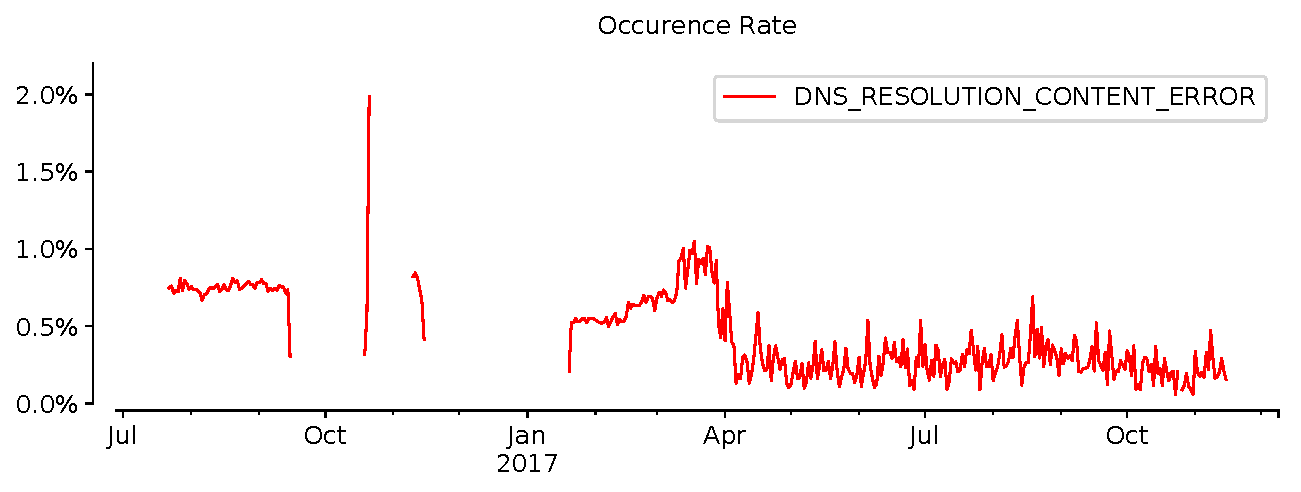
\includegraphics[keepaspectratio, height=3cm, width=7.5cm]{figures/errors/netflix-occurence-rate-dns-content.pdf}
		\caption[Occurrence Rate DNS Resolution Content Error]{(a)}
		\label{fig:Occurrence Rate DNS Resolution Content Error}
	\end{minipage}
	\begin{minipage}{0.50\textwidth}
		\centering
		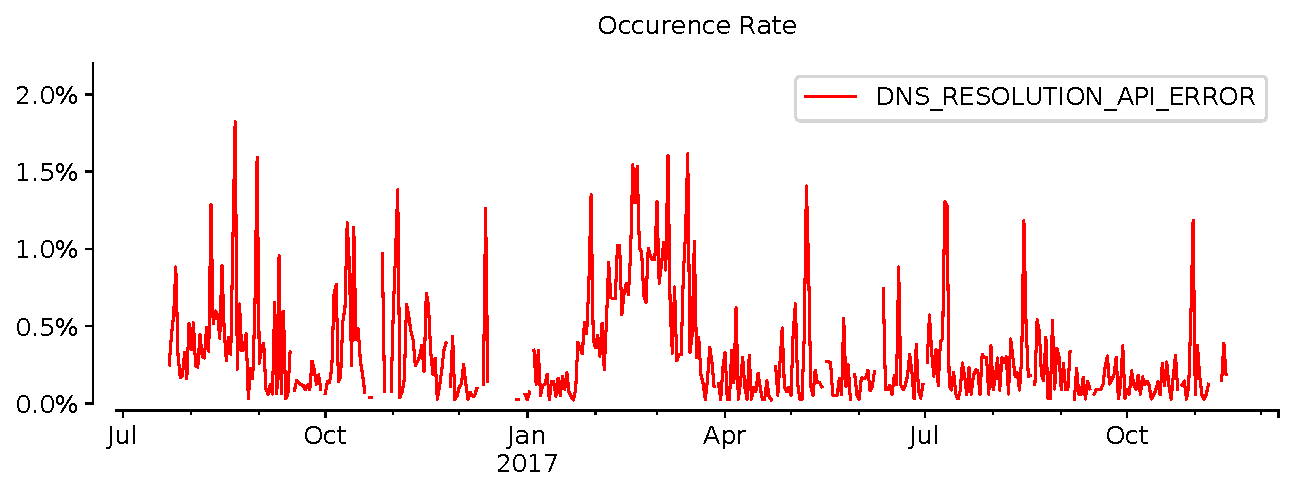
\includegraphics[keepaspectratio, height=3cm, width=7.5cm]{figures/errors/netflix-occurence-rate-dns-api.pdf}
		\caption[Occurrence Rate DNS Resolution API Error]{(b)}
		\label{fig:Occurrence Rate DNS Resolution API Error}
	\end{minipage}
	\begin{minipage}{0.5\textwidth}
		\centering
		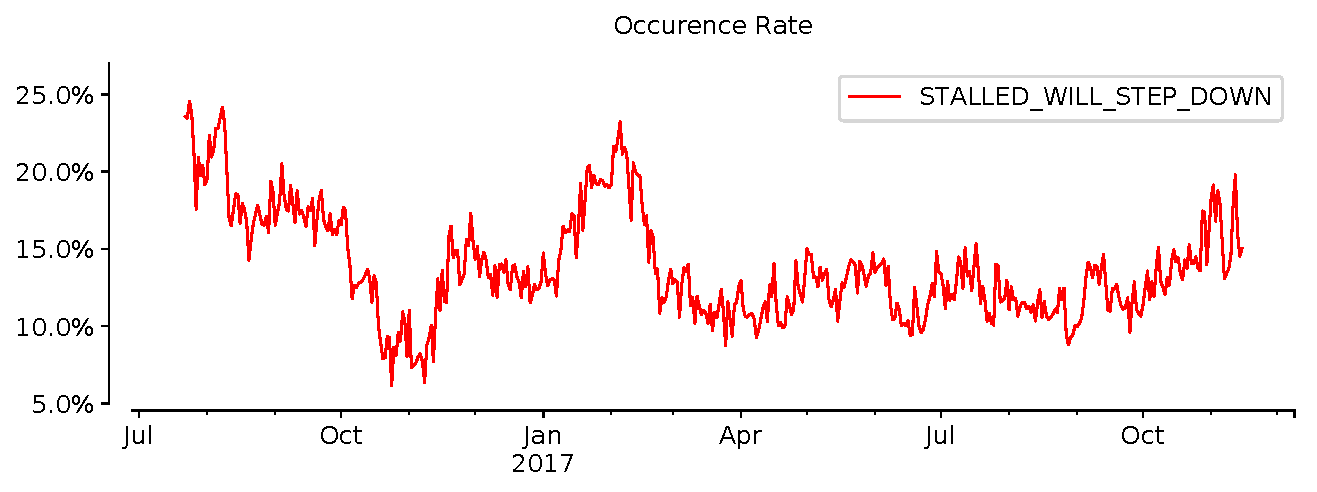
\includegraphics[keepaspectratio, height=3cm, width=7.5cm]{figures/errors/netflix-occurence-rate-stalled-will.pdf}
		\caption[Occurrence Rate Stalled Will Step Down Error]{(c)}
		\label{fig:Occurrence Rate Stalled Will Step Down Error}
	\end{minipage}
	\begin{minipage}{0.5\textwidth}
		\centering
		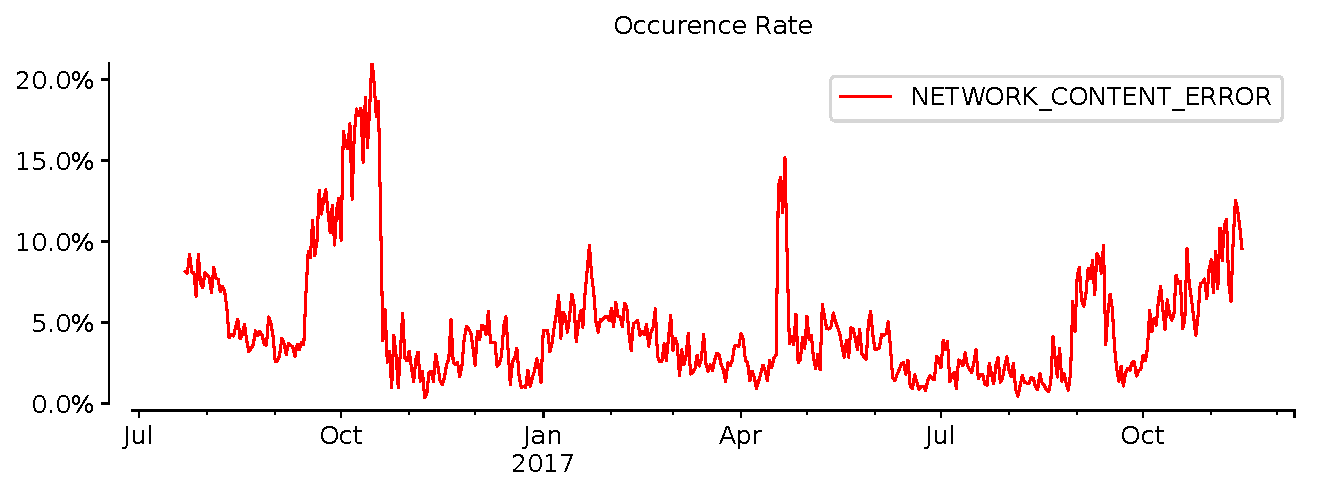
\includegraphics[keepaspectratio, height=3cm, width=7.5cm]{figures/errors/netflix-occurence-rate-network-content.pdf}
		\caption[Occurrence Rate Network Content Error]{(d)}
		\label{fig:Occurrence Rate Network Content Error}
	\end{minipage}
	\begin{minipage}{0.5\textwidth}
		\centering
		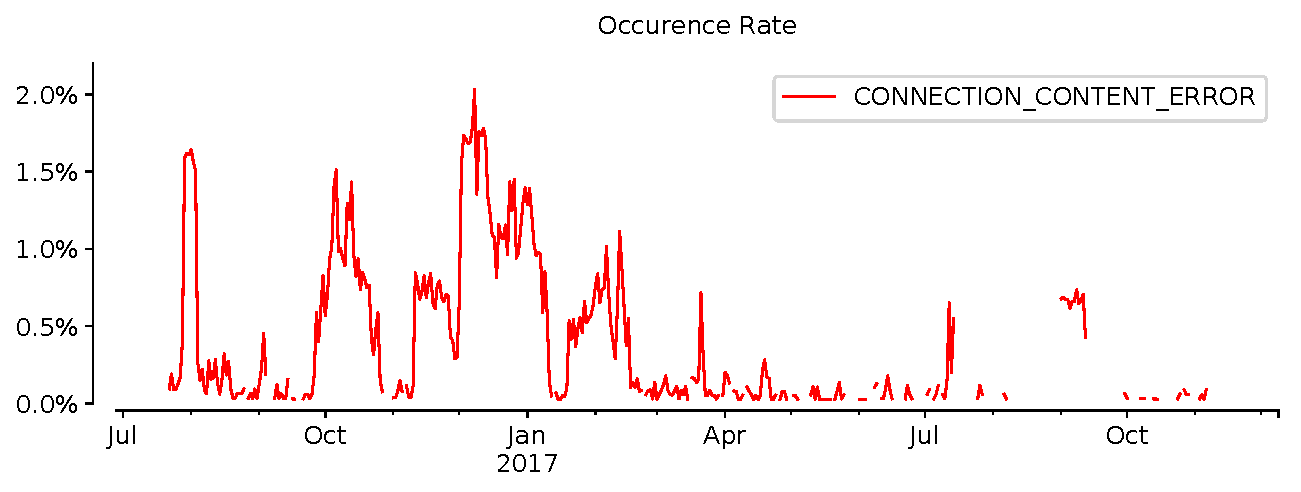
\includegraphics[keepaspectratio, height=3cm, width=7.5cm]{figures/errors/netflix-occurence-rate-connection-content.pdf}
		\caption[Occurrence Rate Connection Content Error]{(e)}
		\label{fig:Occurrence Rate Connection Content Error}
	\end{minipage}
	\begin{minipage}{0.5\textwidth}
		\centering
		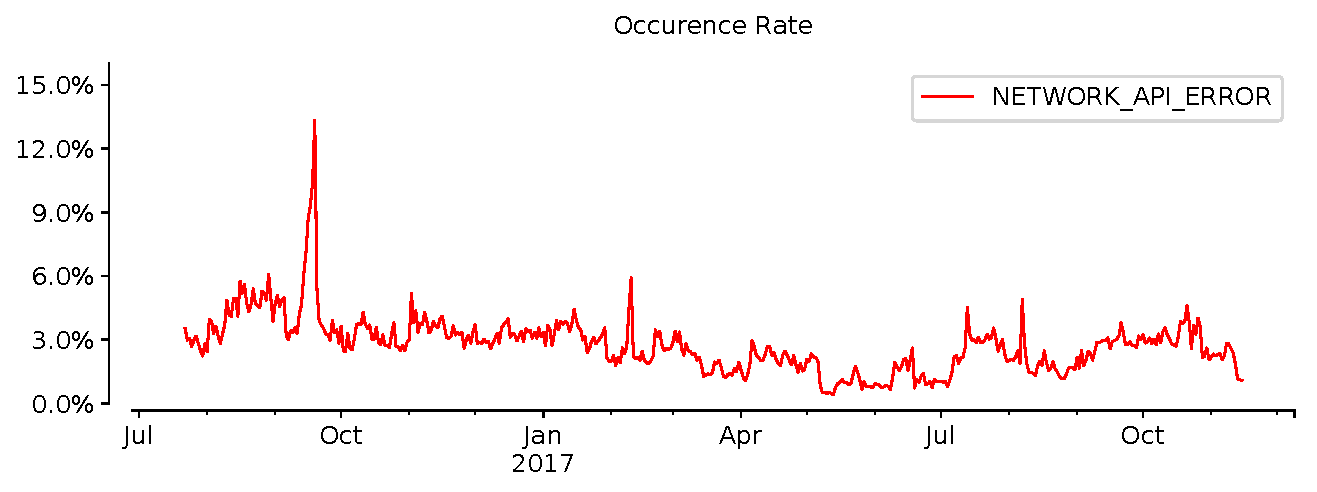
\includegraphics[keepaspectratio, height=3cm, width=7.5cm]{figures/errors/netflix-occurence-rate-network-api.pdf}
		\caption[Occurrence Rate Network API Error]{(f)}
		\label{fig:Occurrence Rate Network API Error}
	\end{minipage}
	\begin{minipage}{0.5\textwidth}
		\centering
		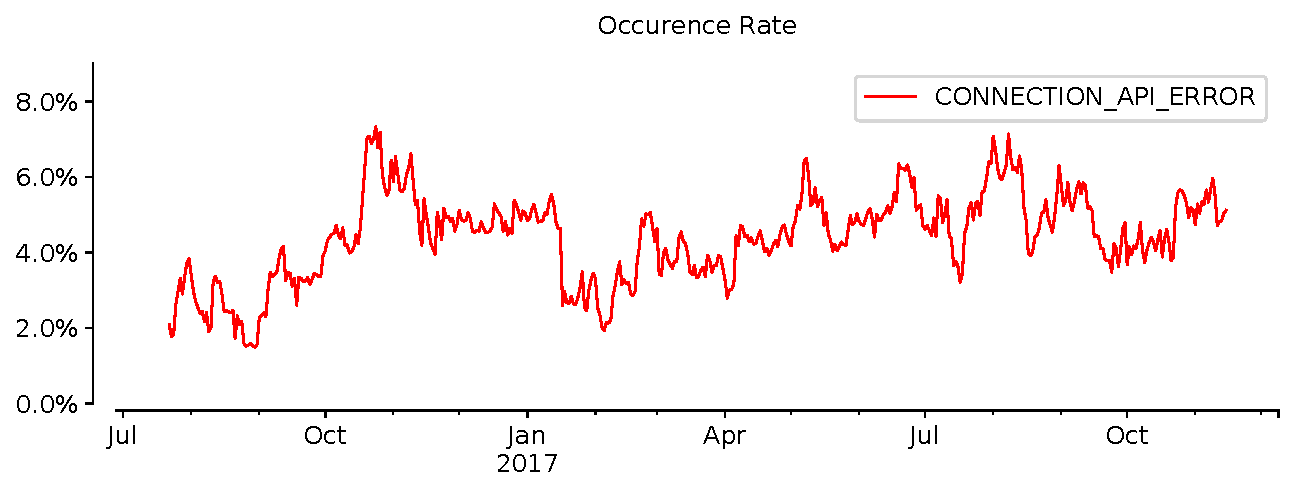
\includegraphics[keepaspectratio, height=3cm, width=7.5cm]{figures/errors/netflix-occurence-rate-connection-api.pdf}
		\caption[Occurrence Rate Connection API Error]{(g)}
		\label{fig:Occurrence Rate Connection API Error}
	\end{minipage}
	\begin{minipage}{0.5\textwidth}
		\centering
		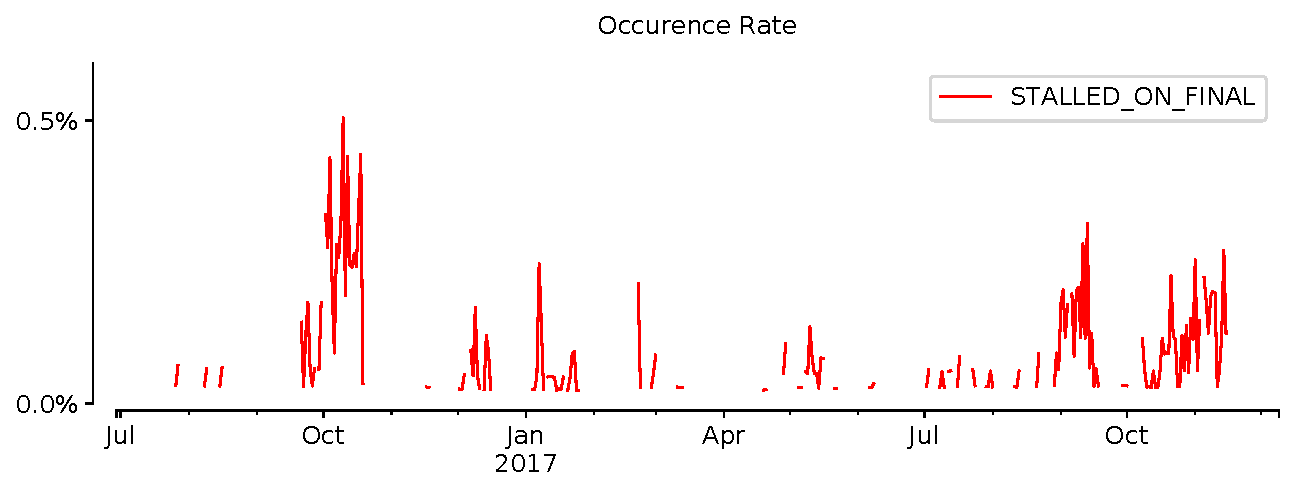
\includegraphics[keepaspectratio, height=3cm, width=7.5cm]{figures/errors/netflix-occurence-rate-stalled-on-final.pdf}
		\caption[Occurrence Rate Stalled On Final Error]{(h)}
		\label{fig:Occurrence Rate Stalled On Final Error}
	\end{minipage}
	\caption[Error Occurrence Rate Time series for Each Error]{(a) Error Occurrence Rate for DNS Resolution Content Error, (b) Error Occurrence Rate for DNS Resolution API Error, 
(c) Error Occurrence Rate for Stalled Will Step Down Error, (d) Error Occurrence Rate for Network Content Error, (e) Error Occurrence Rate for Connection Content Error, 
(f) Error Occurrence Rate for Network API Error, (g) Error Occurrence Rate for Connection API Error, (h) Error Occurrence Rate for Stalled On Final Error}
	\label{fig:Error Occurrence Rate Time series for Each Error}
\end{figure}

\FloatBarrier
\subsubsection*{\textit{Success Rate}}

\begin{figure}[!ht]
	\centering
	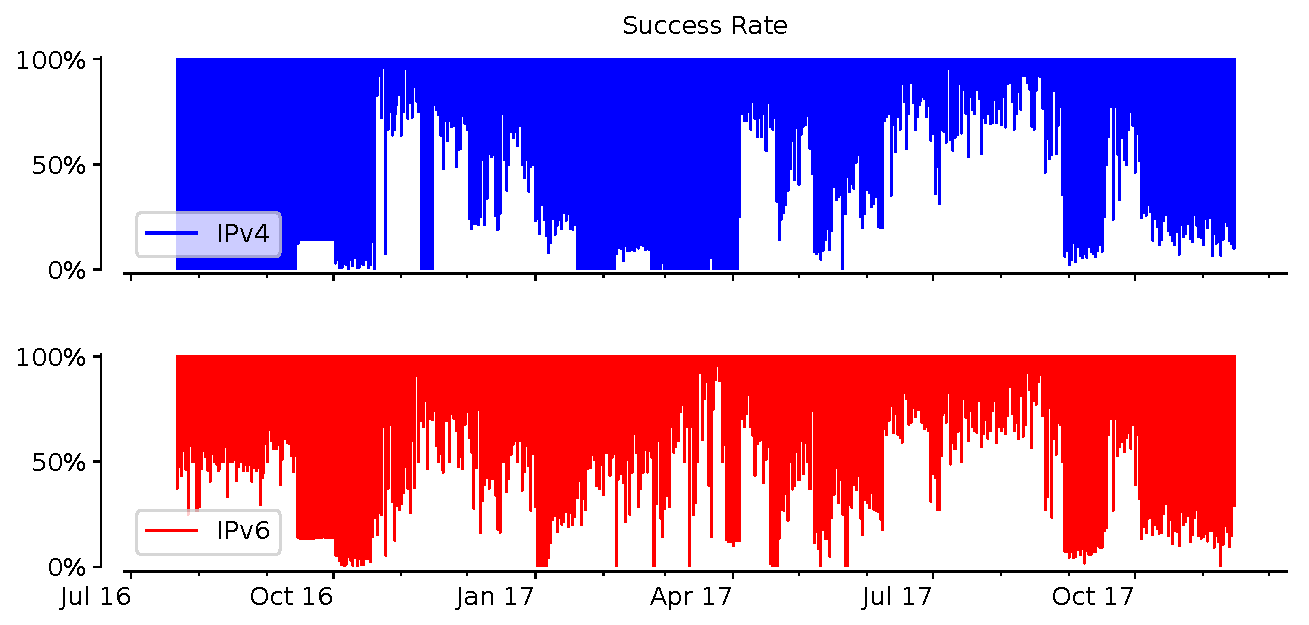
\includegraphics[keepaspectratio, height=4cm, width=15cm]{figures/success/netflix-success-rate-timeseries-no-median.pdf}
	\caption[Success Rate Timeseries all datapoints]{Time series of success rate over IPv4 and IPv6. We are plotting all the datapoints and not just the median aggregate as in \cref{fig:Success Rate Timeseries}. IPv4 shows lower success rate of many days over the timeline.}
	\label{fig:Success Rate Timeseries all datapoints}
\end{figure}
\begin{figure}[!ht]
	\centering
	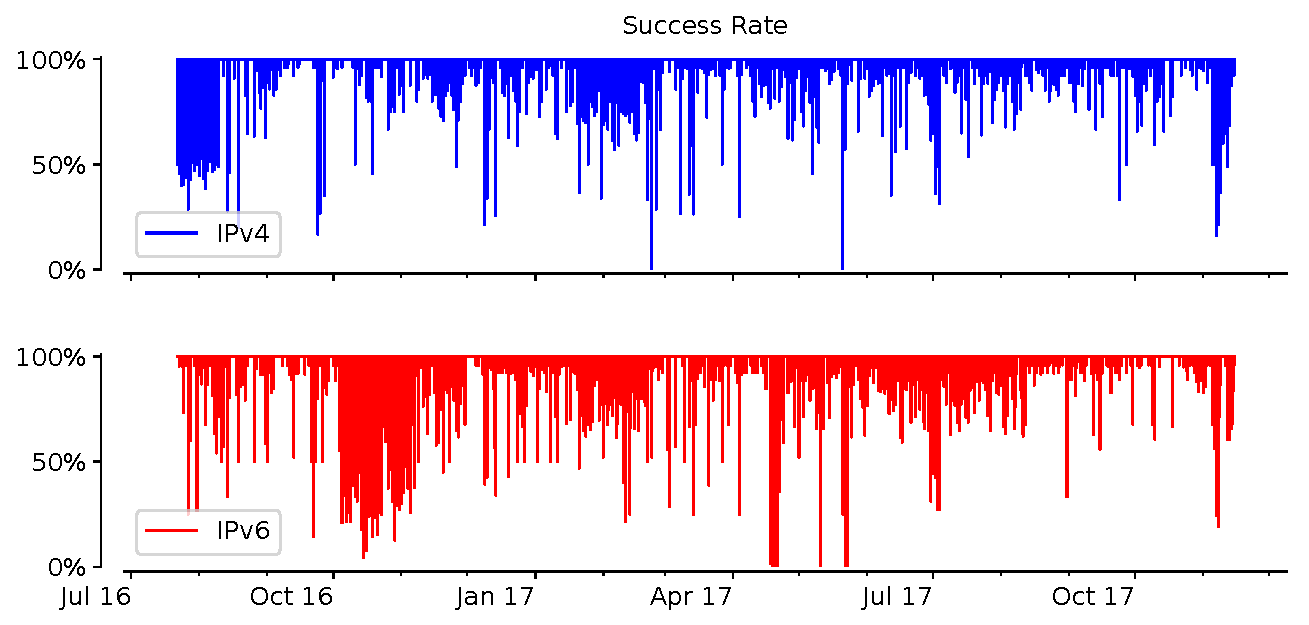
\includegraphics[keepaspectratio, height=4cm, width=15cm]{figures/success/netflix-success-rate-timeseries-no-median-outlier.pdf}
	\caption[Success Rate Timeseries all data points without Outliers]{Time series of success rate over IPv4 and IPv6, removing the 30 probes based on \cref{fig:Error Occurrence and Success Rate by Each Probe}(b).}
	\label{fig:Success Rate Timeseries all datapoints wihout Outliers}
\end{figure}
As already discussed in \cref{chapter:esrate}, we are comparing the success rate over IPv4 and IPv6. \cref{fig:Success Rate Timeseries all datapoints} depicts the time series of 
success rate
when we are plotting all the data points and not just the median aggregate across all probes on each day as in \cref{fig:Success Rate Timeseries}. We can see from the density that the success rate over IPv4 is lower for many days along the timeline. We now remove 30 probes based on \cref{fig:Error Occurrence and Success Rate by Each Probe}(b) which have a lower success rate over both the families.
\begin{figure}[!ht]
	\centering
	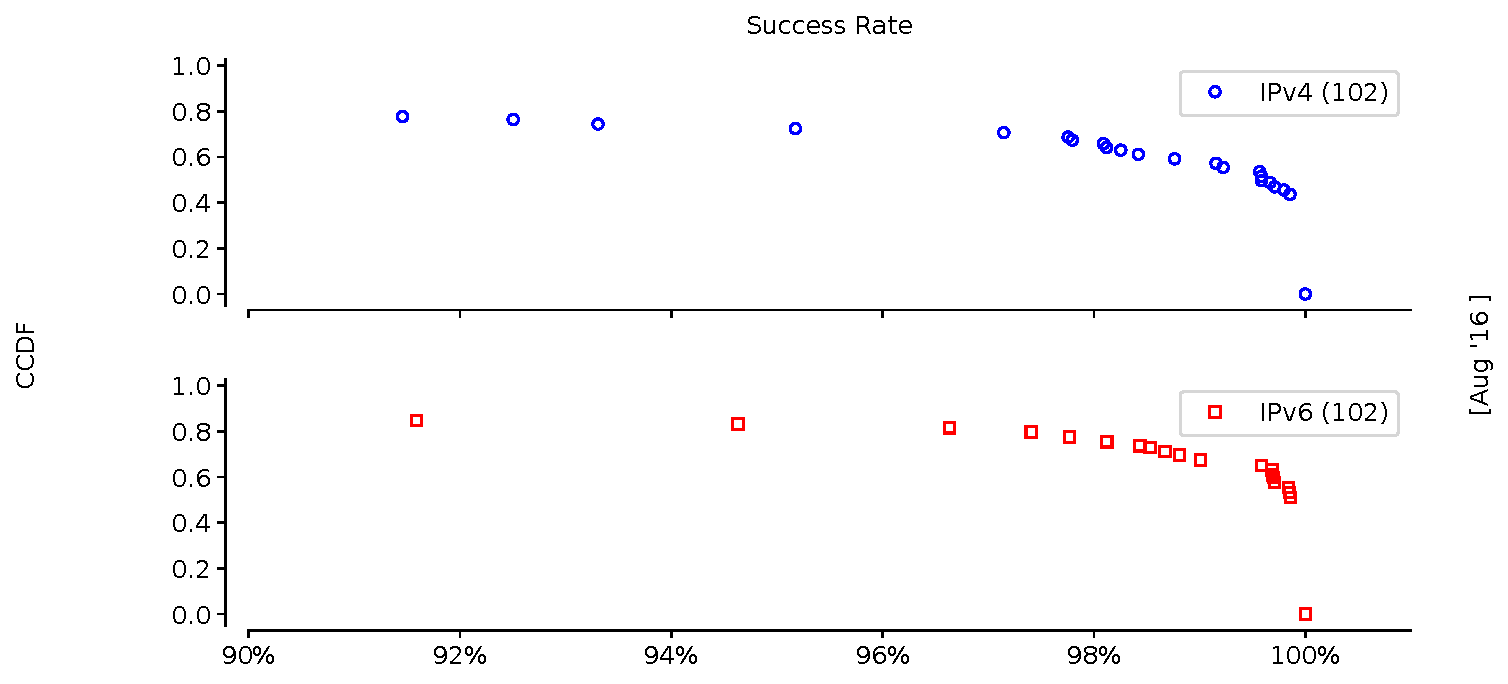
\includegraphics[keepaspectratio, height=4cm, width=15cm]{figures/success/netflix-success-rate-ccdf-aug-2016.pdf}
	\caption[Success Rate CCDF for August 2016]{CCDF of success rate over IPv4 and IPv6 for August 2016. Around 71\% of the probes achieve a success rate of more than 97\% over IPv4, whereas for IPv6 80\% of the probes were able to achieve the success rate.}
	\label{fig:Success Rate for August 2016}
\end{figure}
\cref{fig:Success Rate Timeseries all datapoints wihout Outliers} shows us the time series after removing these outliers. As can be seen both the families show similar spikes, 
depicting lower success rates on some days.
\cref{fig:Success Rate for August 2016} and \cref{fig:Success Rate CCDF for October 2017} depicts the CCDF of success rate over IPv4 and IPv6 for the month of August 2016 and 
October 2017 respectively.
For August 2016, around 71\% of the probes achieve a success rate of more than 97\% over IPv4, whereas for IPv6 80\% of the probes were able to achieve the success rate.
For October 2017, around 88\% of the probes achieve a success rate of more than 97\% over IPv4, whereas for IPv6 90\% of the probes were able to achieve the same success rate.
\cref{fig:Success Rate boxplot for each day of the week} shows the boxplot over each day of the week. The success rate is 100\% over each day of the week when there isn't a stall happening.
\begin{figure}[!ht]
	\centering
	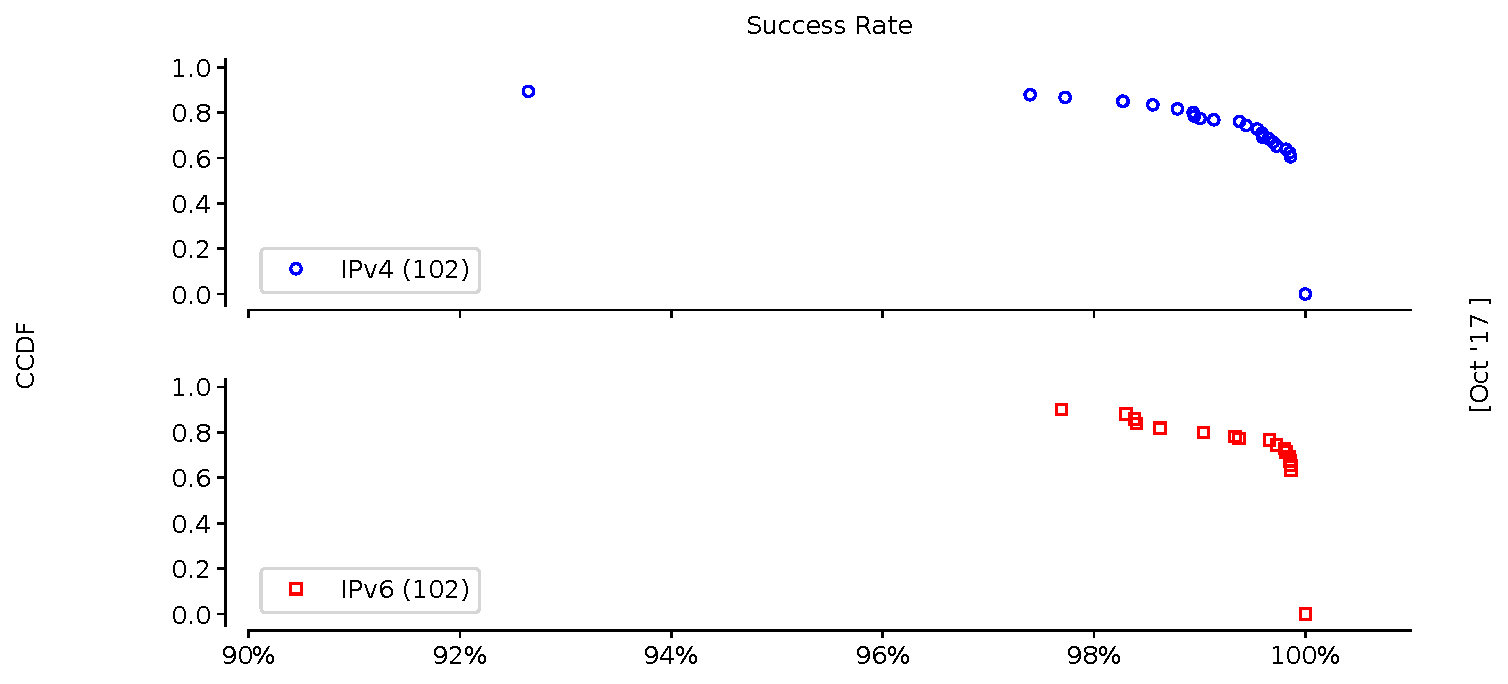
\includegraphics[keepaspectratio, height=4cm, width=15cm]{figures/success/netflix-success-rate-ccdf-oct-2017.pdf}
	\caption[Success Rate CCDF for Ocotber 2017]{CCDF of success rate over IPv4 and IPv6 for October 2017. Around 88\% of the probes achieve a success rate of more than 97\% over IPv4, whereas for IPv6 90\% of the probes were able to achieve the same success rate.}
	\label{fig:Success Rate CCDF for October 2017}
\end{figure}
\begin{figure}[!ht]
	\centering
	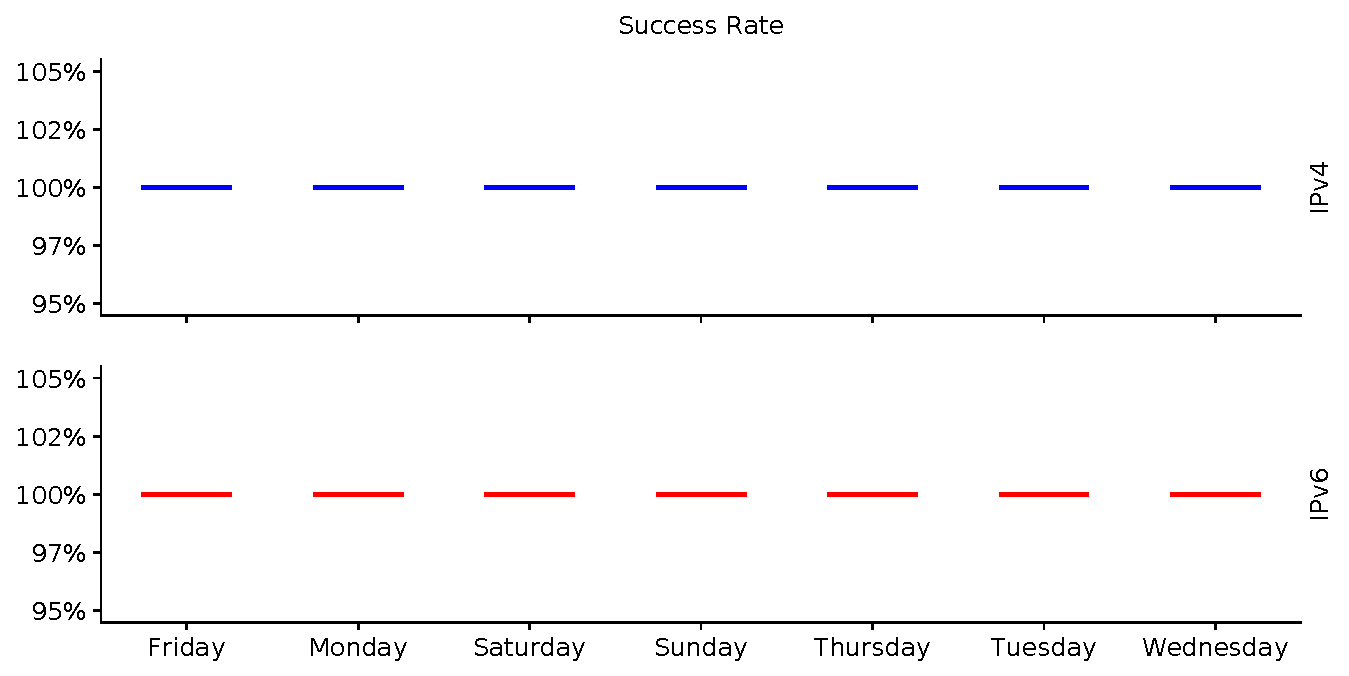
\includegraphics[keepaspectratio, height=4cm, width=15cm]{figures/success/netflix-success-rate-boxplot-days.pdf}
	\caption[Success Rate Boxplot for each day of the week]{Boxplot of success rate over IPv4 and IPv6 by each day of the week. Success rate is 100\% over each day of the week.}
	\label{fig:Success Rate boxplot for each day of the week}
\end{figure}
\vspace{\fill}
\FloatBarrier
\subsection{IPv6 Preference}
\begin{figure}[!ht]
	\centering
	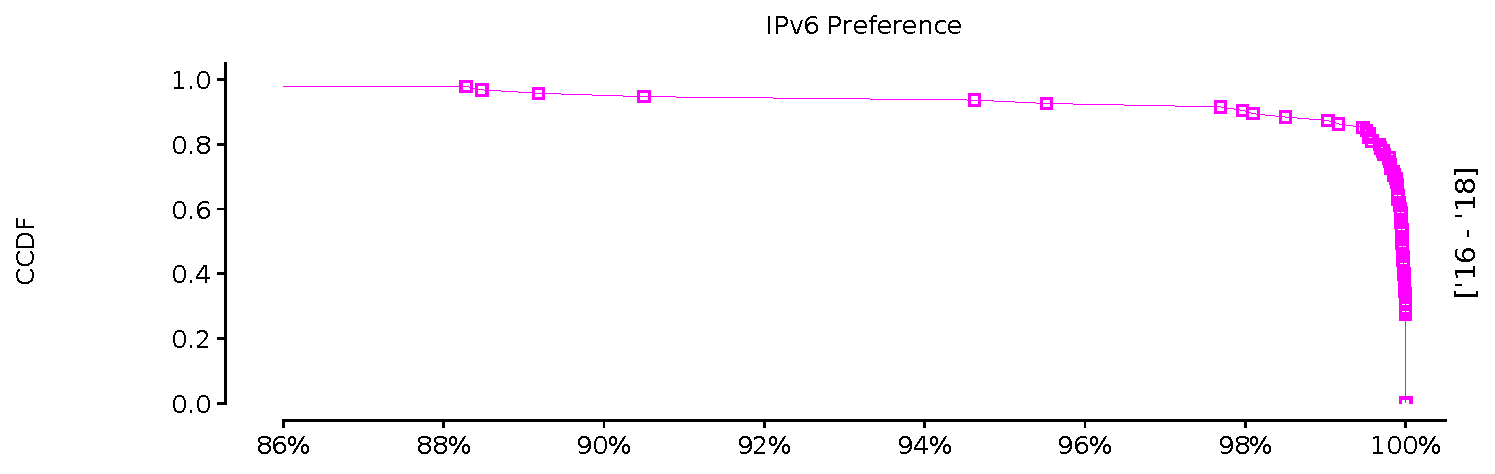
\includegraphics[keepaspectratio, height=4cm, width=15cm]{figures/preference/he-preference-ccdf-target.pdf}
	\caption[IPv6 Preference CCDF by Probes]{CCDF of TCP connect time over IPv6 group by probes. Here, TCP connections over IPv6 were preferred for at-least 88\% of the time.}
	\label{fig:IPv6 Preference CCDF by Probes}
\end{figure}

This is in continuation to what we discussed in section \ref{chapter:ipv6preference}. The effects of HE algorithm \cite{rfc6555} can be seen in \cref{fig:IPv6 Preference CCDF by Probes}, and as per that when we cluster the data by probes after calculating the preference, the TCP connect times over IPv6 are preferred for at-least 88\% of the time.
\FloatBarrier
\subsection{Latency and Delays}
\begin{figure}[!ht]
	\centering
	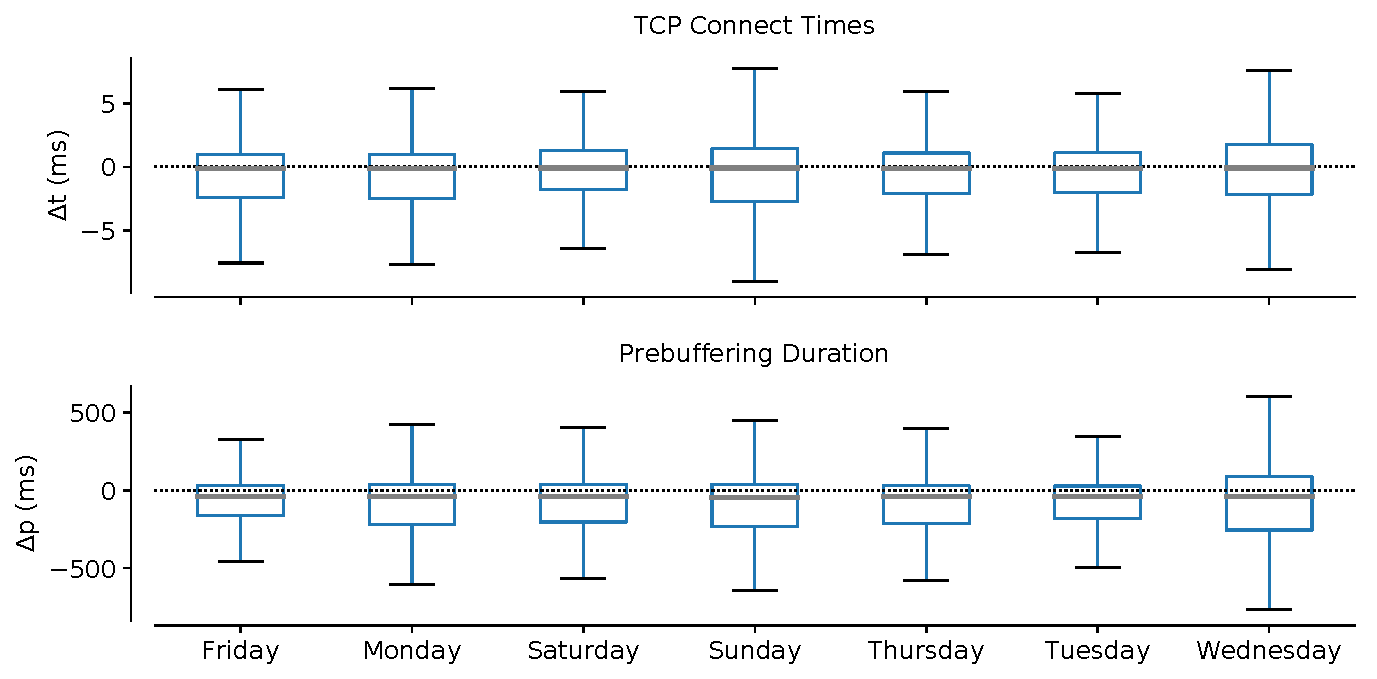
\includegraphics[keepaspectratio, height=4cm, width=15cm]{figures/tcp/netflix-connect-time-pd-boxplot-day.pdf}
	\caption[TCP Connect Times and Prebuffering Duration Boxplot for each Day of the Week]{}
	\label{fig:TCP Connect Times and Prebuffering Duration Boxplot for each Day of the Week}
\end{figure}

We continue our discussion regarding latency and delays, \cref{fig:TCP Connect Times and Prebuffering Duration Boxplot for each Day of the Week} shows us the TCP connect times and prebuffering duration to Netflix OCAs for each day of the week. We can see that the latency and delays are consistent during over all the days of the week.  

\FloatBarrier

\subsection{Benifits of ISP Content Caches}

\subsection*{British Telecommunications (BT) }

\subsubsection*{TCP Latency and Delay}

\begin{figure}[!ht]
	\centering
	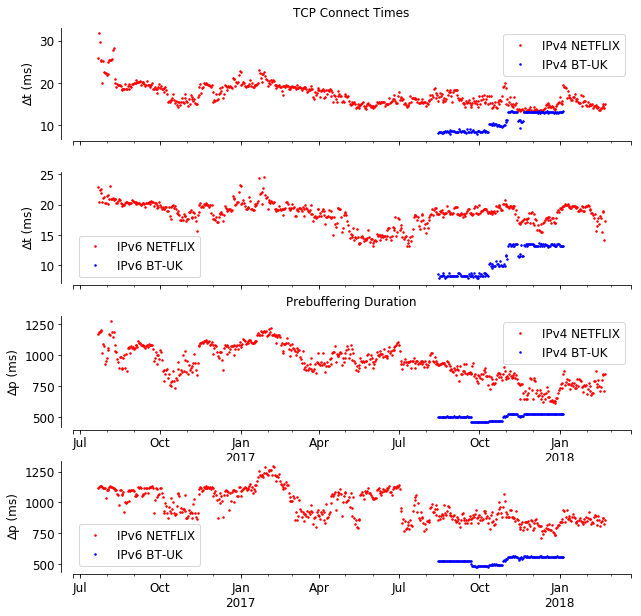
\includegraphics[keepaspectratio, height=8cm, width=15cm]{figures/cache/btuk/netflix-tcp-pd-delay-timeseries-asn-2856-separate.png}
	\caption[BT-UK TCP Connect Times and Pre-Buffering Duration Timeseries Absolute]{Timeseries depicting the TCP connect times (\textit{connect\_time} field) and Prebuffering Duration (\textit{prebuffering\_duration} field) for BT against Netflix OCA servers. 
	We are applying a median aggregate here over the absolute values and as can be seen, the TCP connect times are better for BT for both the address families. Prebuffering duration also shows the similar results.}
	\label{fig:BT-UK TCP Connect Times and Pre-Buffering Duration Timeseries Absolute}
\end{figure}

\begin{figure}[!ht]
	\centering
	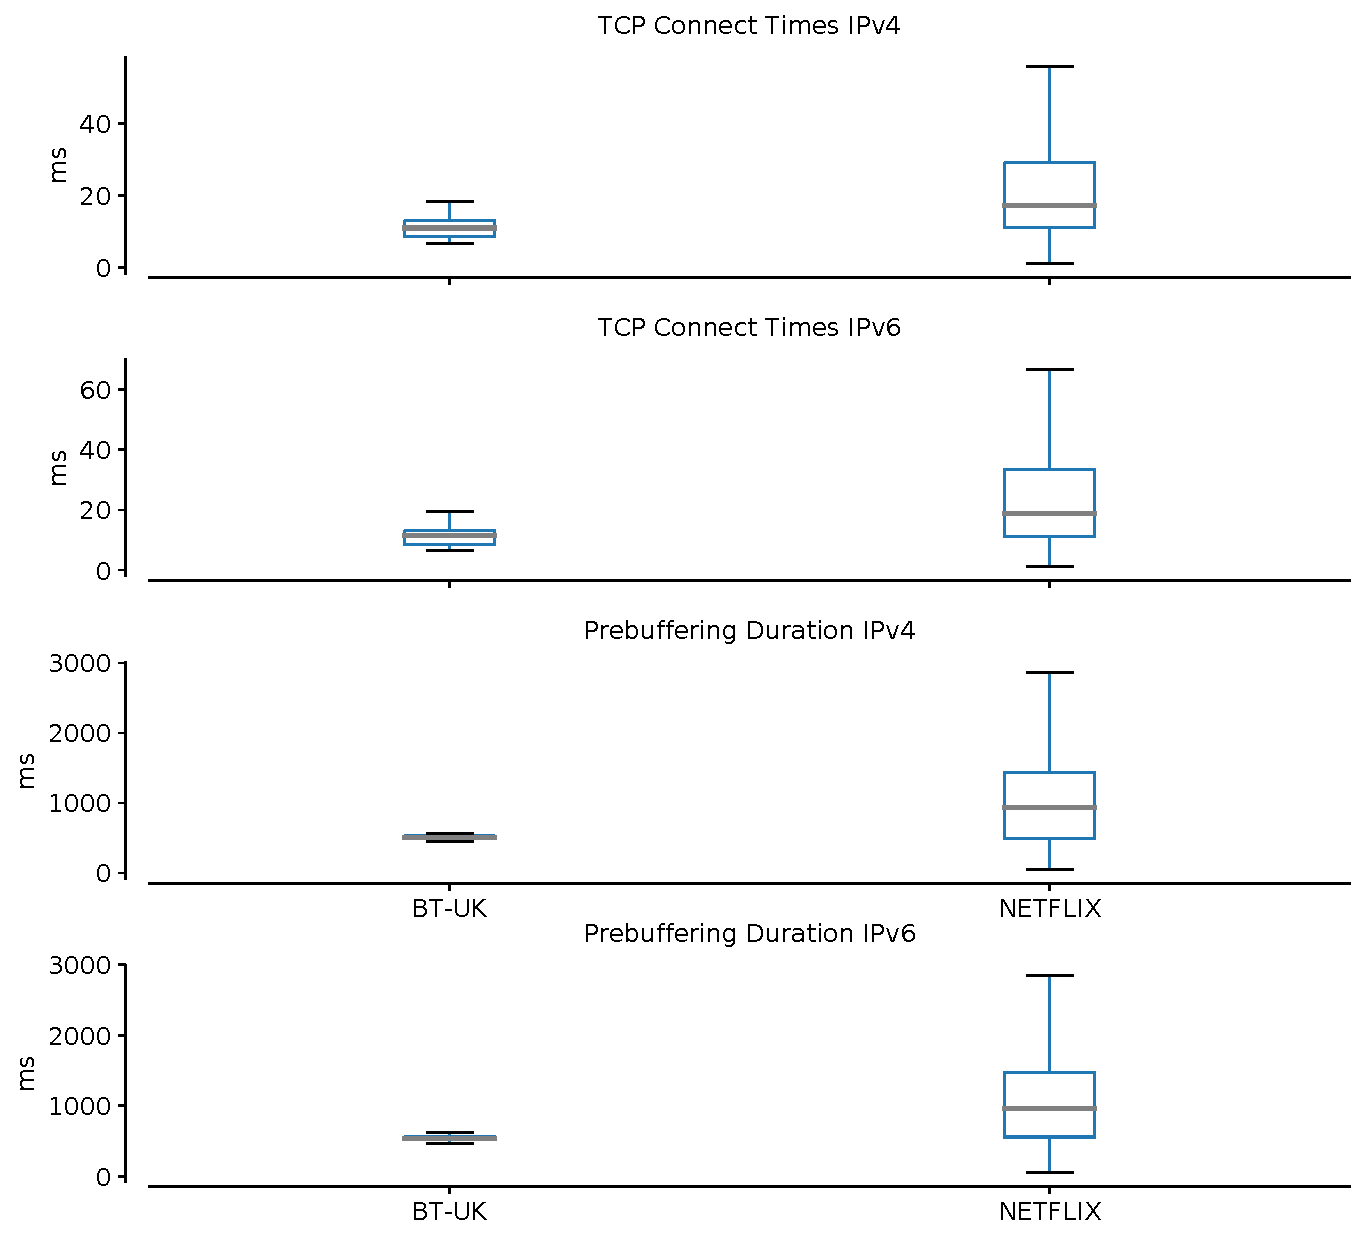
\includegraphics[keepaspectratio, height=8cm, width=15cm]{figures/cache/btuk/netflix-tcp-prebuffering-delay-boxplot-btuk-seprate.pdf}
	\caption[BT-UK TCP Connect Times and Pre-Buffering Duration Boxplot Absolute]{Boxplot depicting TCP connect times and Pre-Bufferring Duration for BT and Netflix. 
	The median resembles the Time series graph in \cref{fig:BT-UK TCP Connect Times and Pre-Buffering Duration Timeseries Absolute}.}
	\label{fig:BT-UK TCP Connect Times and Pre-Buffering Duration Boxplot Absolute}
\end{figure}

\textit{British Telecommunications (BT)} has the AS Number 2856, so for filtering out the rows which are using the criteria was, both AS number of source IP address and AS number of destination IP address belongs to
the same AS number which is 2856 here. Here, we are considering the \textit{connect\_time} and \textit{prebuffering\_duration} fields that are defined in \cref{table:netflix}. We first wanted to see how 
TCP connect times and pre-buffering durations perform for both ISP caches and for Netflix (AS number 2906).
\cref{fig:BT-UK TCP Connect Times and Pre-Buffering Duration Timeseries Absolute} shows the timeseries for BT content caches and Netflix OCA servers over both the address families and we have a group by \textit{dtime} field and are considering the median aggregate here so that a single vantage point doesn't bias the results.
As we can see, the TCP connect times is better for BT for both the address families, i.e. (0-15 ms), whereas for Netflix its around (0-30 ms). Pre-buffering duration also shows the similar
results. We have converted the connect time and pre-buffering duration to 'ms' to get a better understanding.
To get a more clear view of the delays, we plot the boxplots for both BT and Netflix over IPv4 and IPv6.  The median line in \cref{fig:BT-UK TCP Connect Times and Pre-Buffering Duration Boxplot Absolute}
graph resembles the timeseries in \cref{fig:BT-UK TCP Connect Times and Pre-Buffering Duration Timeseries Absolute}. Furthermore, the third quartile is pretty low for \textit{British Telecommunications} content caches.
We further investigate the distribution of latency and delays for BT and Netflix, here also, we filter the data along IPv4 and IPv6 and then take the CDF of the desired attributes. 
\cref{fig:BT-UK Connect Time and Prebuffering Duration CDF Absolute} shows the CDF of TCP connect times and pre-buffering durations for BT and Netflix. Around 80\% of the probes require TCP connect times of 13ms
for BT over IPv4, whereas it's 38 ms for the same number of probes for Netflix. Similarly, for IPv6, 80\% of the probes require 13 ms for BT, whereas it is 40ms for Netflix.
For the pre-buffering duration, BT caches require around 527ms for 80\% of the probes over IPv4, and for Netflix the number is 1661 ms for the same number of probes. For IPv6, BT requires
559 ms for 80\% of the probes and for Netflix the number is 1730 ms. It would be also good to compare the deltas i.e. the difference between the Latencies over IPv4 and IPv6 for BT and Netflix.
\begin{figure}
	\centering
	\begin{minipage}{0.5\textwidth}
		\centering
		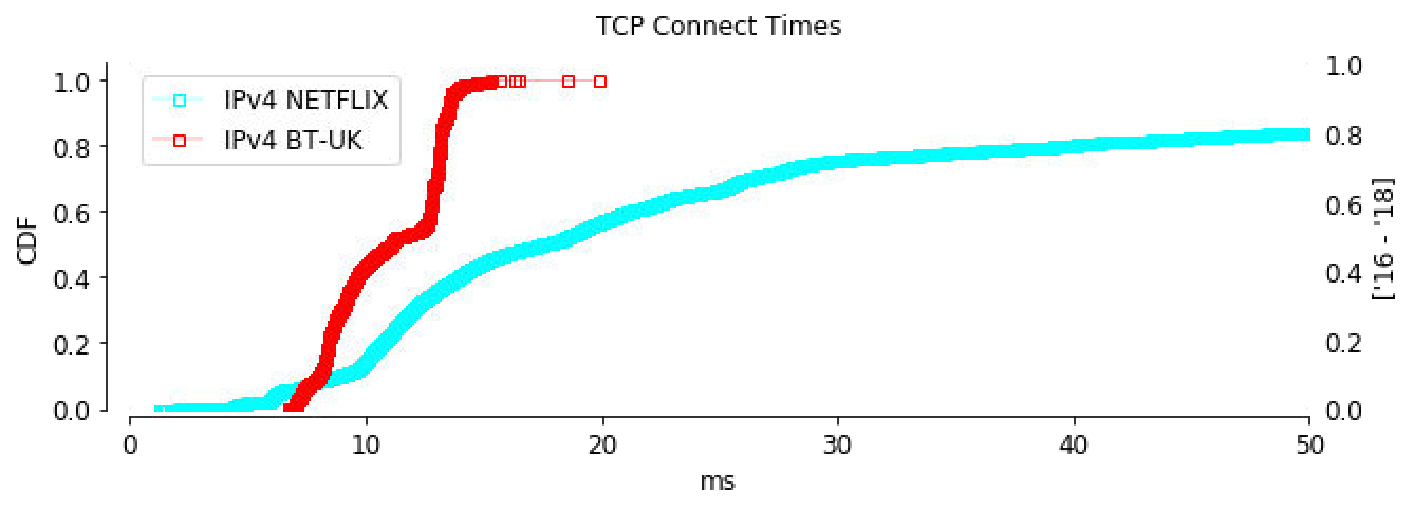
\includegraphics[keepaspectratio, height=5cm, width=8.5cm]{figures/cache/btuk/netflix-syn-time-separate-btuk-v4.pdf}
	\end{minipage}
	\begin{minipage}{0.5\textwidth}
		\centering
		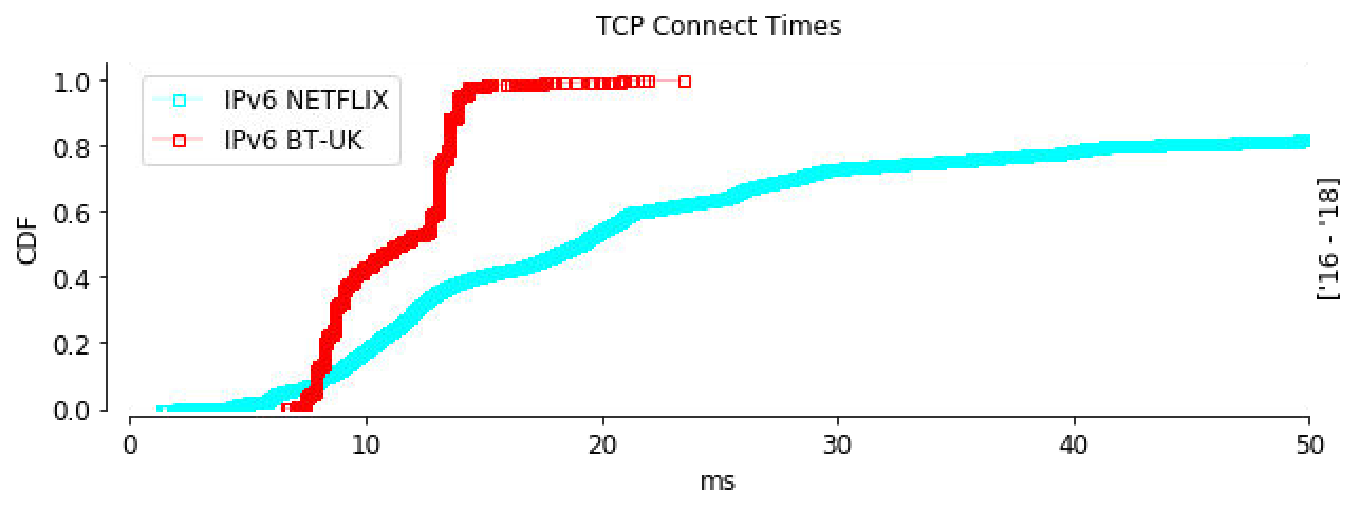
\includegraphics[keepaspectratio, height=5cm, width=8.5cm]{figures/cache/btuk/netflix-syn-time-separate-btuk-v6.pdf}
	\end{minipage}
	\begin{minipage}{0.5\textwidth}
		\centering
		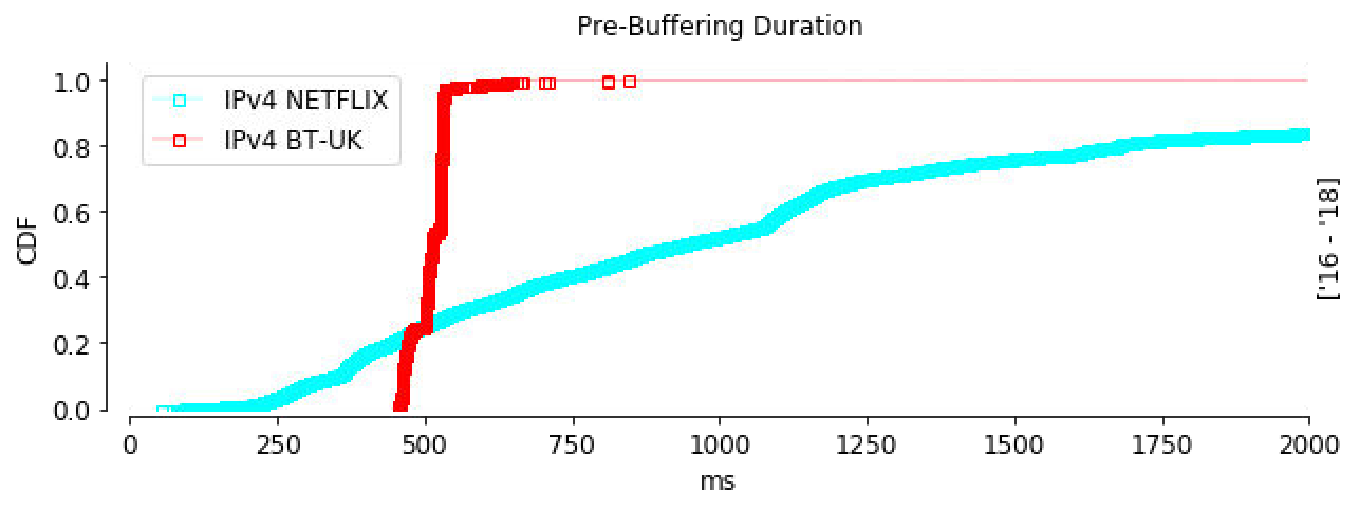
\includegraphics[keepaspectratio, height=5cm, width=8.5cm]{figures/cache/btuk/netflix-prebuffering-duration-separate-btuk-v4.pdf}
	\end{minipage}
	\begin{minipage}{0.5\textwidth}
		\centering
		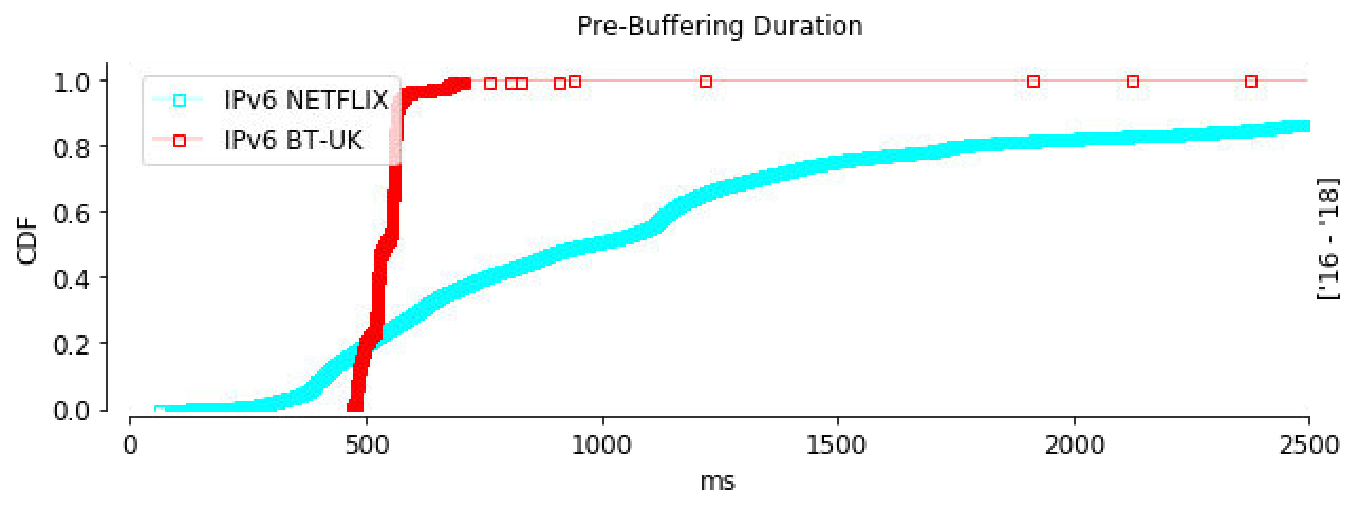
\includegraphics[keepaspectratio, height=5cm, width=8.5cm]{figures/cache/btuk/netflix-prebuffering-duration-separate-btuk-v6.pdf}
	\end{minipage}
	\caption[BT-UK Connect Time and Prebuffering Duration CDF Absolute]{CDF of TCP Connect times and Pre-Buffering duration for BT and Netflix over IPv4 and IPv6. As we can see, TCP Connect times and Prebuffering duration for BT content caches is better than Netflix OCA servers.}
	\label{fig:BT-UK Connect Time and Prebuffering Duration CDF Absolute}
\end{figure}

\FloatBarrier

We will now compare the Deltas that is, the difference between Netflix OCA server TCP connect times and BT caches TCP connect times over IPv4 and IPv6. We will now define the
terminology that we are using here, let us say, TCP connect time over IPv4 for BT is tp(y) and TCP connect time over IPv4 for Netflix is tp(x), then the \textit{delta} will be $\Delta$tp = tp(x) - tp(y). 
We did calculate these deltas for TCP connect times and Pre-buffering duration for BT and Netflix over IPv4 and IPv6.
Also, as already discussed in \cref{chapter:Datasets}, pre-buffering duration takes into account DNS resolution times and TCP connect times. 
We will now analyse the deltas to check the benefits of ISP caches.

\begin{figure}[!ht]
	\centering
	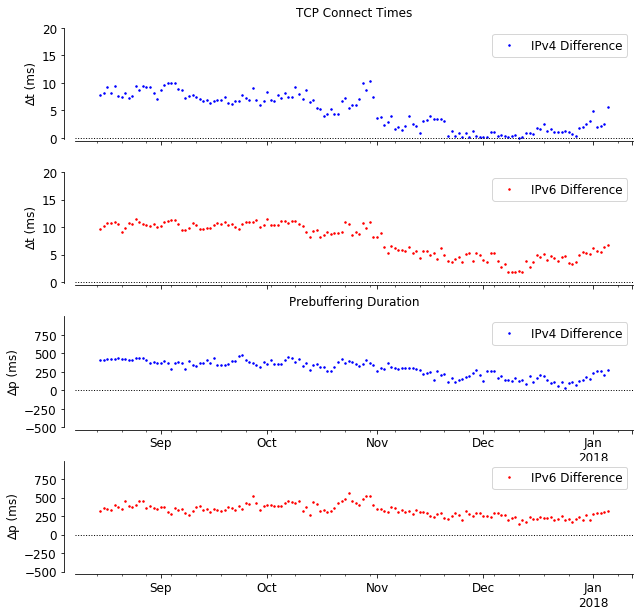
\includegraphics[keepaspectratio, height=8cm, width=15cm]{figures/cache/btuk/netflix-tcp-pd-delay-timeseries-asn-2856.png}
	\caption[BT-UK TCP Connect Times and Pre-Buffering Duration Timeseries Deltas]{Time series of difference for TCP connect times and prebuffering durations over IPv4 and IPv6 between Netflix and BT. 
	Here, positive values indicate Netflix OCA server requires more connect time and pre-buffering duration as compared to BT caches. A latency of around 10-15 ms and higher pre-buffering durations (around 0-500 ms or more) are observed for Netflix over both IPv4 and IPv6.}
	\label{fig:BT-UK TCP Connect Times and Pre-Buffering Duration Timeseries Deltas}
\end{figure}

\begin{figure}[!ht]
	\centering
	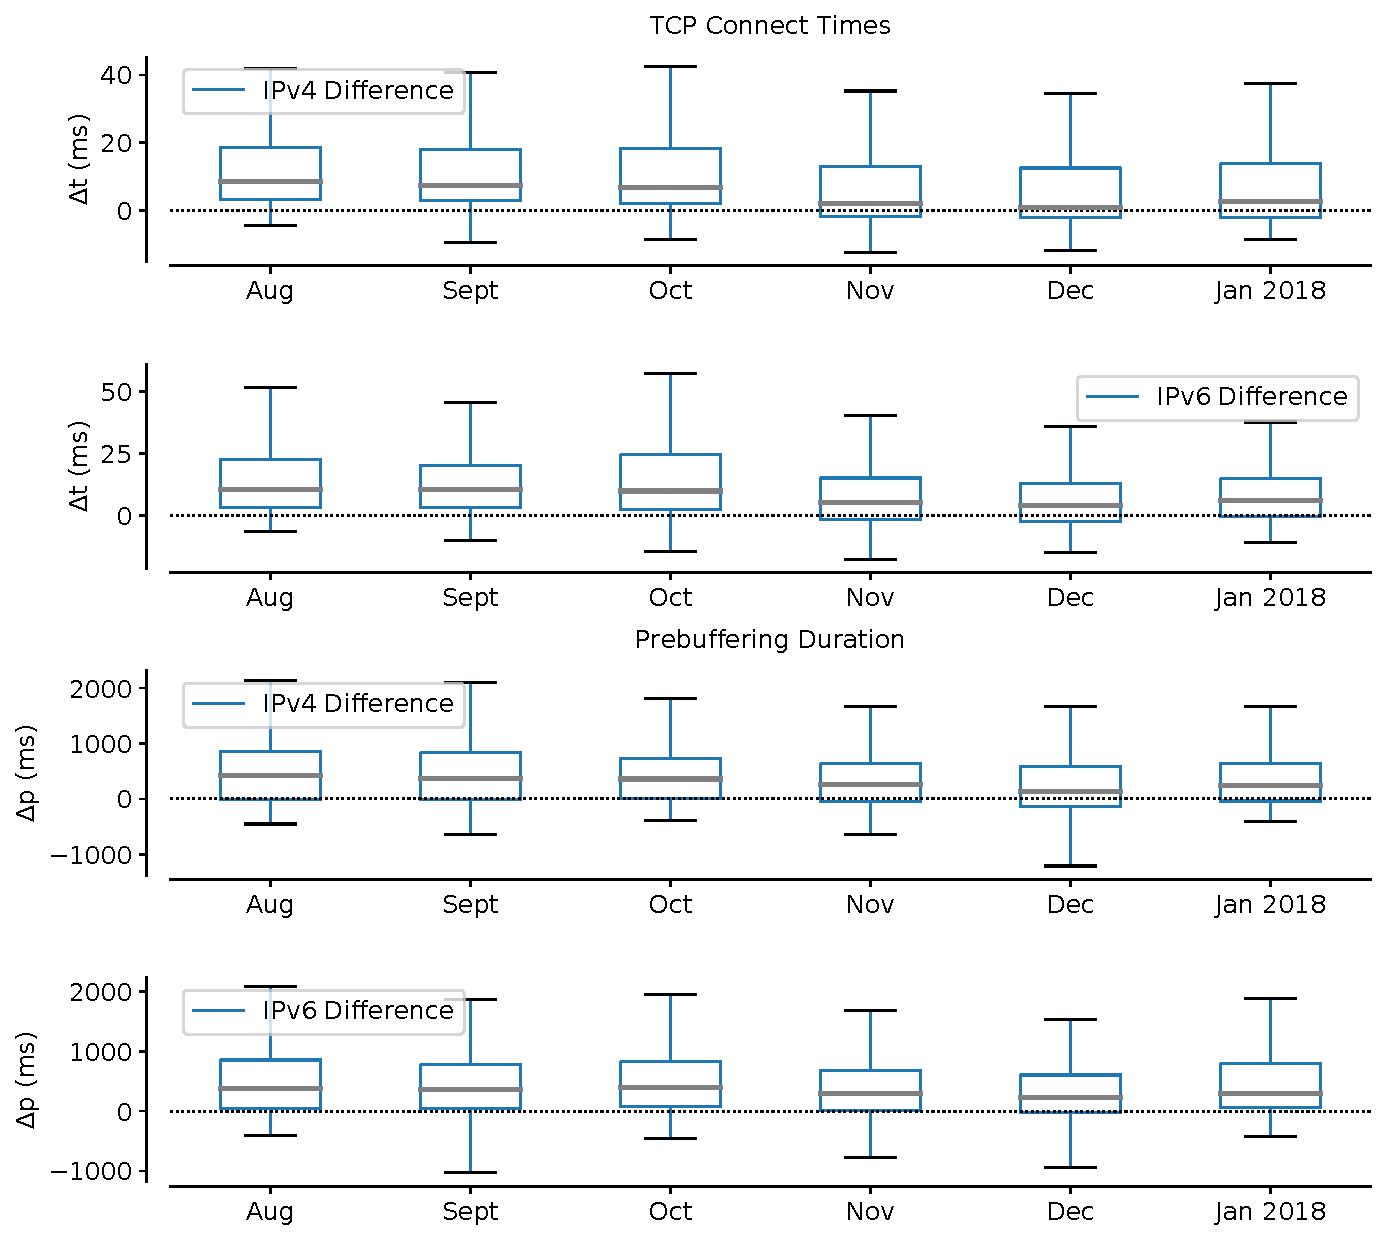
\includegraphics[keepaspectratio, height=8cm, width=15cm]{figures/cache/btuk/netflix-tcp-pd-delay-boxplot-asn-2856.pdf}
	\caption[BT-UK TCP Connect Times and Pre-Buffering Duration Boxplot Deltas]{Boxplot of difference for TCP connect times and prebuffering durations over IPv4 and IPv6 between Netflix and SKY UK Limited.
	The median line here represents the time series graph in \cref{fig:BT-UK TCP Connect Times and Pre-Buffering Duration Timeseries Deltas}.}
	\label{fig:BT-UK TCP Connect Times and Pre-Buffering Duration Boxplot Deltas}
\end{figure}

To plot the deltas, we followed the same analysis \cite{bajpaimeasuring} did for the Youtube dataset. To plot the timeseries for these deltas, we calculate the median aggregate on the
TCP connect times and the prebuffering duration across all probes on each day for the difference between Netflix and BT.
\cref{fig:BT-UK TCP Connect Times and Pre-Buffering Duration Timeseries Deltas} shows the timeseries of median TCP connect times and pre-buffering duration over IPv4 and IPv6 across all probes.
Here, positive values indicate Netflix OCA server requires more connect time and pre-buffering duration as compared to BT caches. A latency of around 0-15 ms and higher pre-buffering durations (around 0-500 ms or more) are observed for Netflix over both IPv4 and IPv6.
For boxplots in \cref{fig:BT-UK TCP Connect Times and Pre-Buffering Duration Boxplot Deltas}, we have rounded the time to the nearest month. Here, we can see that the median resembles the time series \cref{fig:BT-UK TCP Connect Times and Pre-Buffering Duration Timeseries Deltas}.
To get more vivid analysis, \cref{fig:BT-UK Connect Time and Prebuffering Duration CDF Deltas} shows us the distribution of the difference in TCP connect times and prebuffering duration over the whole duration.
For calculating the CDF, we calculated the deltas and then plotted their CDF. To compare the performance, 
we are measuring the TCP connect times to the Netflix OCA (Open Connect Appliances) server and to the BT content caches, 
the distribution here shows that around 78\% of the connections are slower for Netflix OCA servers over IPv4, and around 79\% of the connections are slower for Netflix over IPv6. 
For pre-buffering duration which is the time to fetch 2 seconds of video at the specified bitrate from the content server, here Netflix OCA (Open Connect Appliances) server and BT caches,
the distribution shows that 71\% of the connections are slower for Netflix over IPv4, and around 78\% of the connections are slower for Netflix over IPv6.

\begin{figure}
	\centering
	\begin{minipage}{0.5\textwidth}
		\centering
		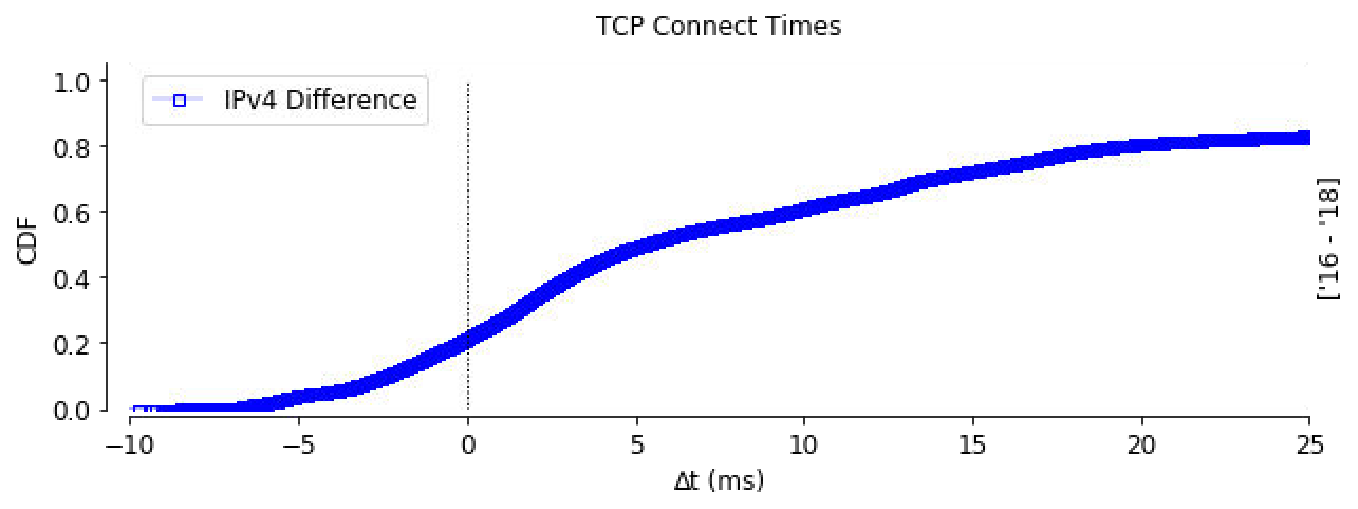
\includegraphics[keepaspectratio, height=5cm, width=8.5cm]{figures/cache/btuk/netflix-syn-diff-2856-cdf-v4.pdf}
	\end{minipage}
	\begin{minipage}{0.5\textwidth}
		\centering
		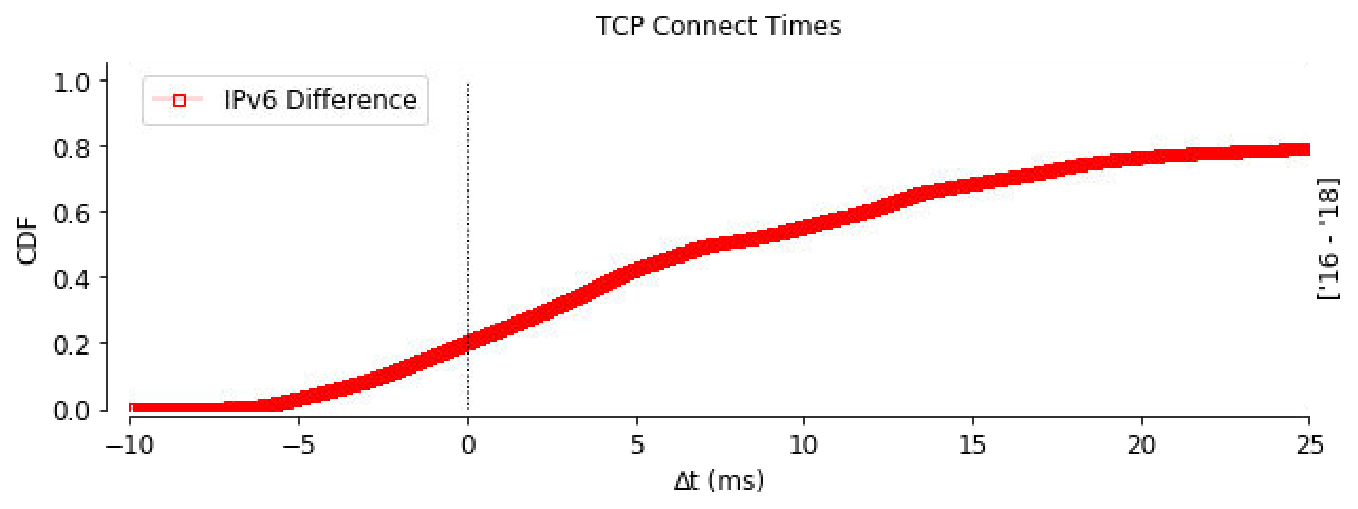
\includegraphics[keepaspectratio, height=5cm, width=8.5cm]{figures/cache/btuk/netflix-syn-diff-2856-cdf-v6.pdf}
	\end{minipage}
	\begin{minipage}{0.5\textwidth}
		\centering
		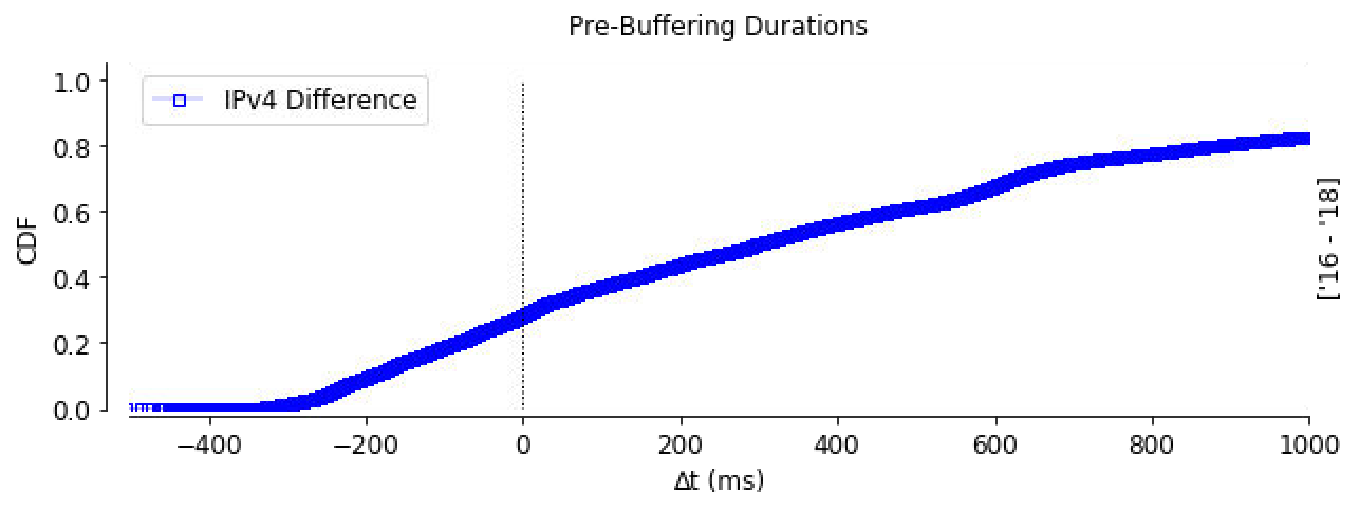
\includegraphics[keepaspectratio, height=5cm, width=8.5cm]{figures/cache/btuk/netflix-pd-diff-2856-cdf-v4.pdf}
	\end{minipage}
	\begin{minipage}{0.5\textwidth}
		\centering
		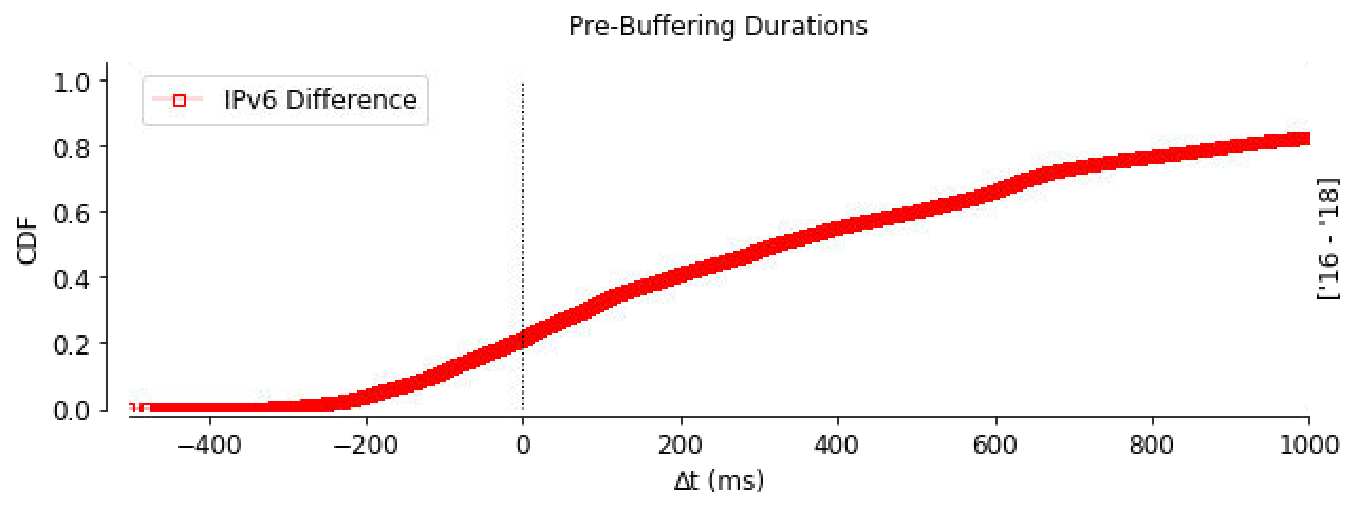
\includegraphics[keepaspectratio, height=5cm, width=8.5cm]{figures/cache/btuk/netflix-pd-diff-2856-cdf-v6.pdf}
	\end{minipage}
	\caption[BT-UK Connect Time and Prebuffering Duration CDF Deltas]{CDF of the difference of TCP connect times and Prebuffering Durations for Netflix and BT over IPv4 and IPv6. The distribution here shows that around 78\% of the connections are slower for Netflix OCA servers over IPv4, and around 79\% of the connections are slower for Netflix over IPv6. 
For pre-buffering duration which is the time to fetch 2 seconds of video at the specified bitrate from the content server, here Netflix OCA (Open Connect Appliances) server and BT caches,
the distribution shows that 71\% of the connections are slower for Netflix over IPv4, and around 78\% of the connections are slower for Netflix over IPv6.}
	\label{fig:BT-UK Connect Time and Prebuffering Duration CDF Deltas}
\end{figure}

\FloatBarrier

\subsubsection*{Throughput}

\begin{figure}[!ht]
	\centering
	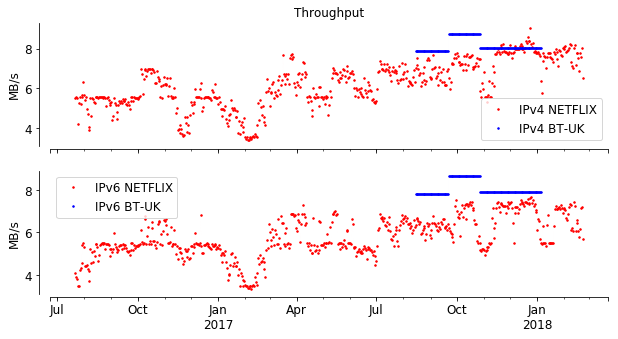
\includegraphics[keepaspectratio, height=5cm, width=15cm]{figures/cache/btuk/netflix-throughput-timeseries-asn-2856-separate.png}
	\caption[BT-UK Throughput Timeseries Absolute]{Time series of Throughput for individual address family's i.e. IPv4 and IPv6 for Netflix and BT. We are considering 
	the \textit{bytes\_sec} field described in \cref{table:netflix}. As can be seen, the achieved throughput for BT caches is somwehat comparable or more than Netflix OCA server.}
	\label{fig:BT-UK Throughput Timeseries Absolute}
\end{figure}

\begin{figure}[!ht]
	\centering
	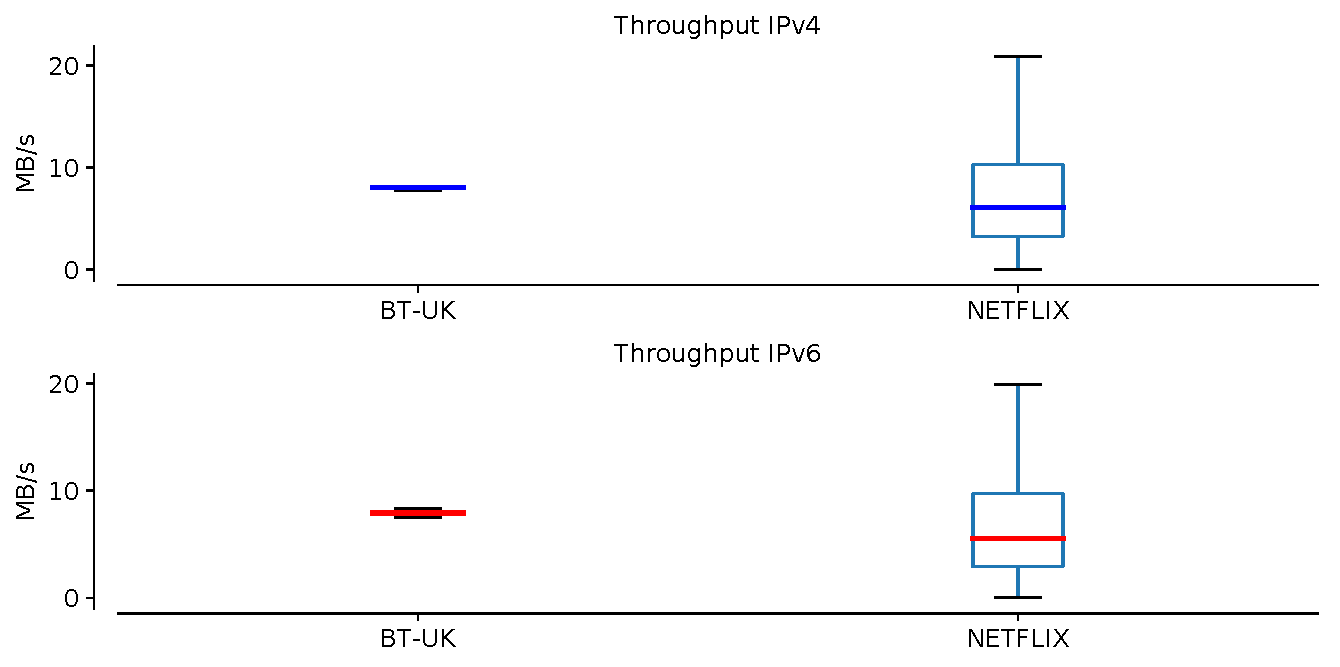
\includegraphics[keepaspectratio, height=5cm, width=15cm]{figures/cache/btuk/netflix-throughput-boxplot-asn-2856-separate.pdf}
	\caption[BT-UK Throughput Boxplot Absolute]{Boxplot of Throughput for individual address family's i.e. IPv4 and Ipv6 for Netflix and BT. The median line here shows that the achieved throughput is
	is higher for BT over both address family's.}
	\label{fig:BT-UK Throughput Boxplot Absolute}
\end{figure}

After comparing the TCP connect times and Pre-Buffering duration for Netflix and BT, we now know that clients take higher TCP connect times and prebuffering duration
for Netflix as compared to the BT caches over both the address families. We will now be comparing the achieved throughput over IPv4 and IPv6 for Netflix OCA server and BT caches.
We will first look into the individual performance of IPv4 and IPv6 for Netflix and BT and we will look into their deltas. \cref{fig:BT-UK Throughput Timeseries Absolute} gives the time series for
both the address families for BT and Netflix, and as can be seen, the achieved throughput for BT caches is more than Netflix OCA server.
We are considering the \textit{bytes\_sec} field from the Netflix \cref{table:netflix}, and we are taking the median aggregate across
all probes on each day. Also, the throughput for IPv4 and IPv6 lies between 7-10 MB/s for BT. To get deeper insights
we also did the boxplot for IPv4 and IPv6 throughput for BT and Netflix, and as can be seen in \cref{fig:BT-UK Throughput Boxplot Absolute} the monthly
throughput variation over IPv4 and IPv6. The median line here shows that the achieved throughput is higher for BT over both address families. We have converted the \textit{bytes\_sec} field into MB/s to get a more realistic view. \cref{fig:BT-UK Throughput CDF Absolute} shows the CDF of
throughput over IPv4 and IPv6. We followed the same steps here and plotted the CDF of \textit{bytes\_sec} field. The CDF here shows that around 80\% of the probes achieved a throughput of 8 MB/s for BT over IPv4, whereas for Netflix this is 11 MB/s
for a similar number of probes. For IPv6, 80\% of the probes achieved the throughput of 8 MB/s, while for Netflix this was 10 MB/s for a similar number of probes. 
We will now look into the deltas to get a better comparison between BT and Netflix. 

\begin{figure}[!ht]
	\centering
	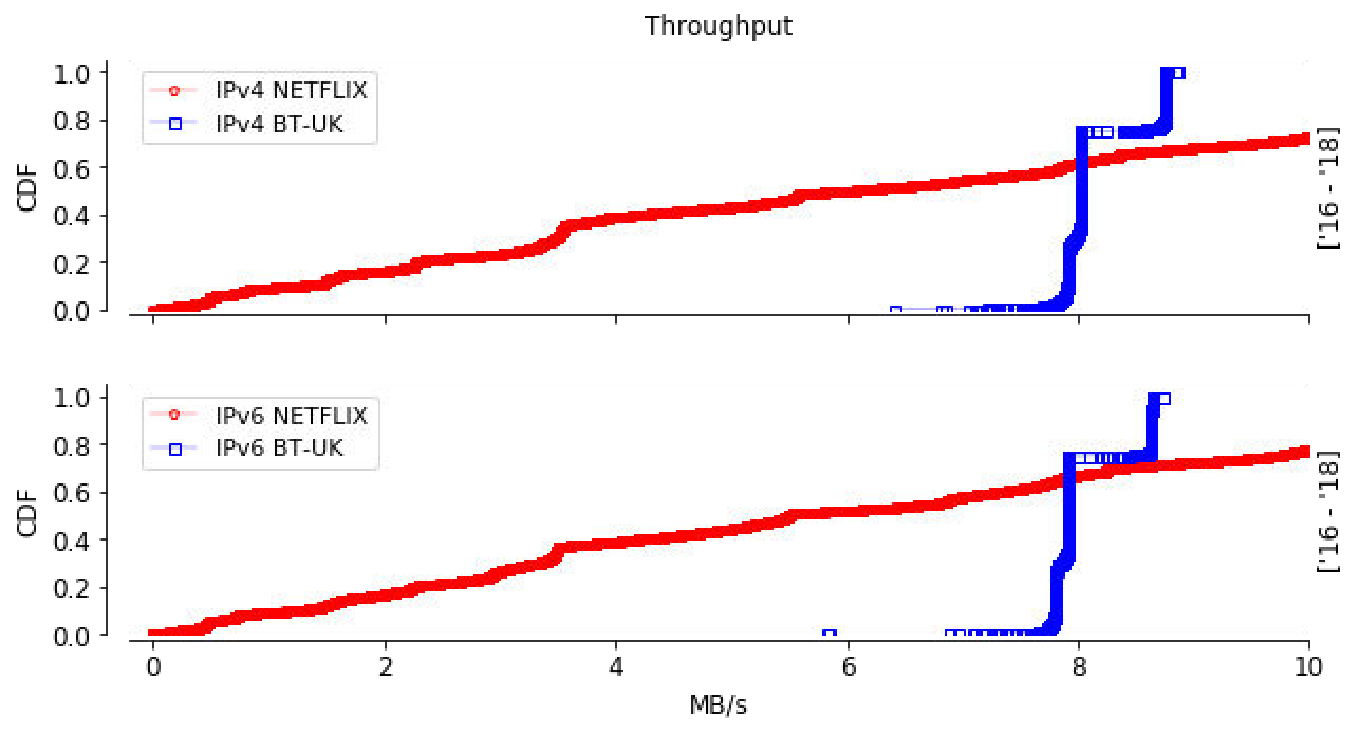
\includegraphics[keepaspectratio, height=5cm, width=15cm]{figures/cache/btuk/netflix-throughput-difference-2856-separate.pdf}
	\caption[BT-UK Throughput CDF Absolute]{CDF of Throughput over IPv4 and IPv6 for BT and Netflix. The CDF here shows that around 80\% of the probes achieved a throughput of 8 MB/s for BT over IPv4, whereas for Netflix this is 11 MB/s
for a similar number of probes. For IPv6, 80\% of the probes achieved the throughput of 8 MB/s, while for Netflix this was 10 MB/s for a similar number of probes.}
	\label{fig:BT-UK Throughput CDF Absolute}
\end{figure}

\FloatBarrier

\begin{figure}[!ht]
	\centering
	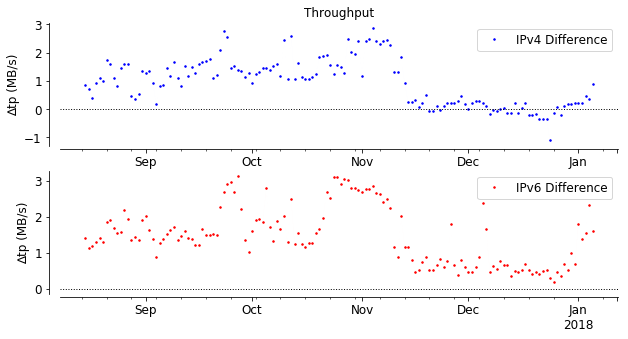
\includegraphics[keepaspectratio, height=5cm, width=15cm]{figures/cache/btuk/netflix-throughput-timeseries-asn-2856.png}
	\caption[BT-UK Throughput Timeseries Deltas]{Time series of deltas of Throughput over IPv4 and IPv6 between BT and Netflix. We can see that the difference is around 0 or more for the whole duration. 
The positive value indicates a higher throughput for BT, also the difference lies between 0-3 MB/s.}
	\label{fig:BT-UK Throughput Timeseries Deltas}
\end{figure}

\begin{figure}[!ht]
	\centering
	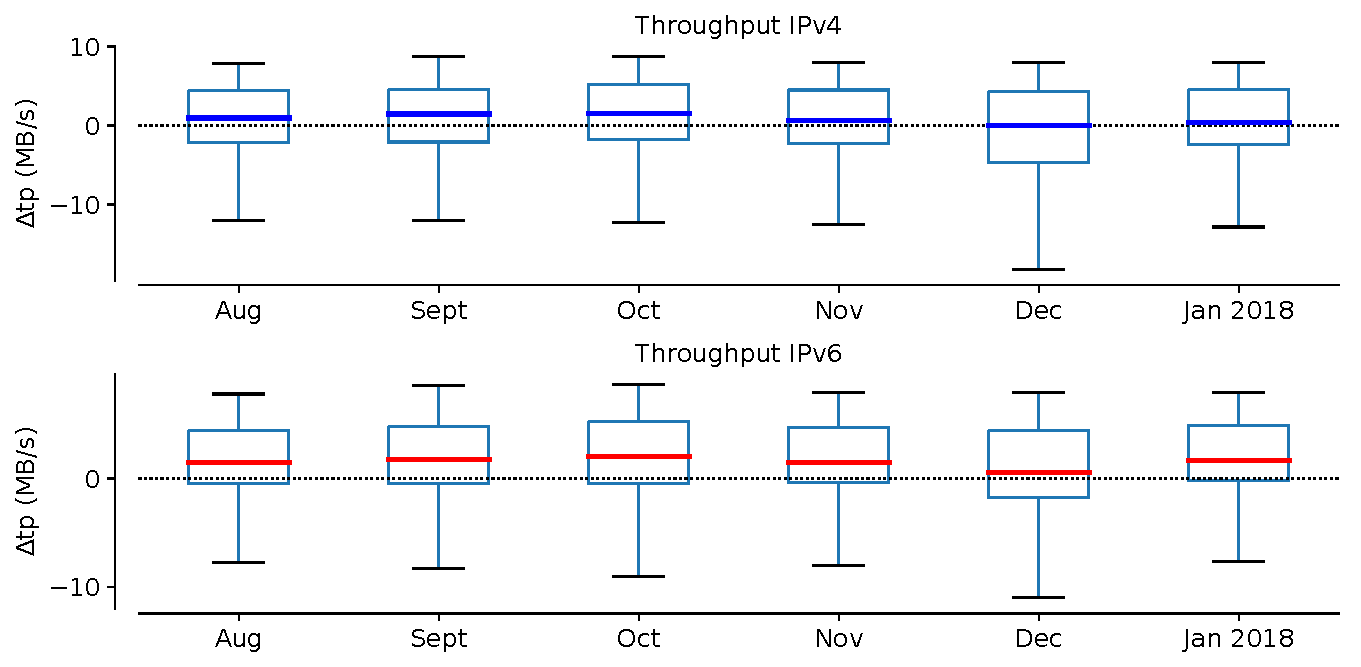
\includegraphics[keepaspectratio, height=5cm, width=15cm]{figures/cache/btuk/netflix-throughput-boxplot-asn-2856.pdf}
	\caption[BT-UK Throughput Boxplot Deltas]{Boxplot of difference of throughput over IPv4 and IPv6 between BT and Netflix. The median line shows similar curves as the time series \cref{fig:BT-UK Throughput Timeseries Deltas}, depicting higher throughput for BT over both address families.}
	\label{fig:BT-UK Throughput Boxplot Deltas}
\end{figure}

Before starting with the deltas, we would like to define the terminologies we used to get the results. We are considering the \textit{bytes\_sec} field only and using the same terminilogy Bajpai et al. used in \cite{bajpaimeasuring}. We denote the throughput 
over IPv4 for BT as \textit{tp(y}) and throughput over IPv4 for Netflix as \textit{tp(x)}, then the \textit{delta} will be $\Delta$tp = tp(y) - tp(x).
To plot the deltas, we first start with the time series, and \cref{fig:BT-UK Throughput Timeseries Deltas} shows us the time series of a median aggregate of throughput across all probes over each day.
We can see that the difference is around 0 or more for the whole duration. The positive value indicates a higher throughput for BT, also the difference lies between 0-3 MB/s.
\cref{fig:BT-UK Throughput Boxplot Deltas} shows the boxplot of the difference of throughput over IPv4 and IPv6 between BT and Netflix. The median line shows similar curves as the time series \cref{fig:BT-UK Throughput Timeseries Deltas}, depicting higher throughput for BT over both address families.
To get a more clear picture of the performance, we plot the CDF of \textit{bytes\_sec} field. 
\cref{fig:BT-UK Throughput CDF Deltas} shows the CDF of the difference of throughput over IPv4 and IPv6 for BT and Netflix. 
Around 59\% of the times, BT caches achieved higher throughput than Netflix over IPv4, and for IPv6 around 69\% of the times, BT caches achieved higher throughput.

\begin{figure}[!ht]
	\centering
	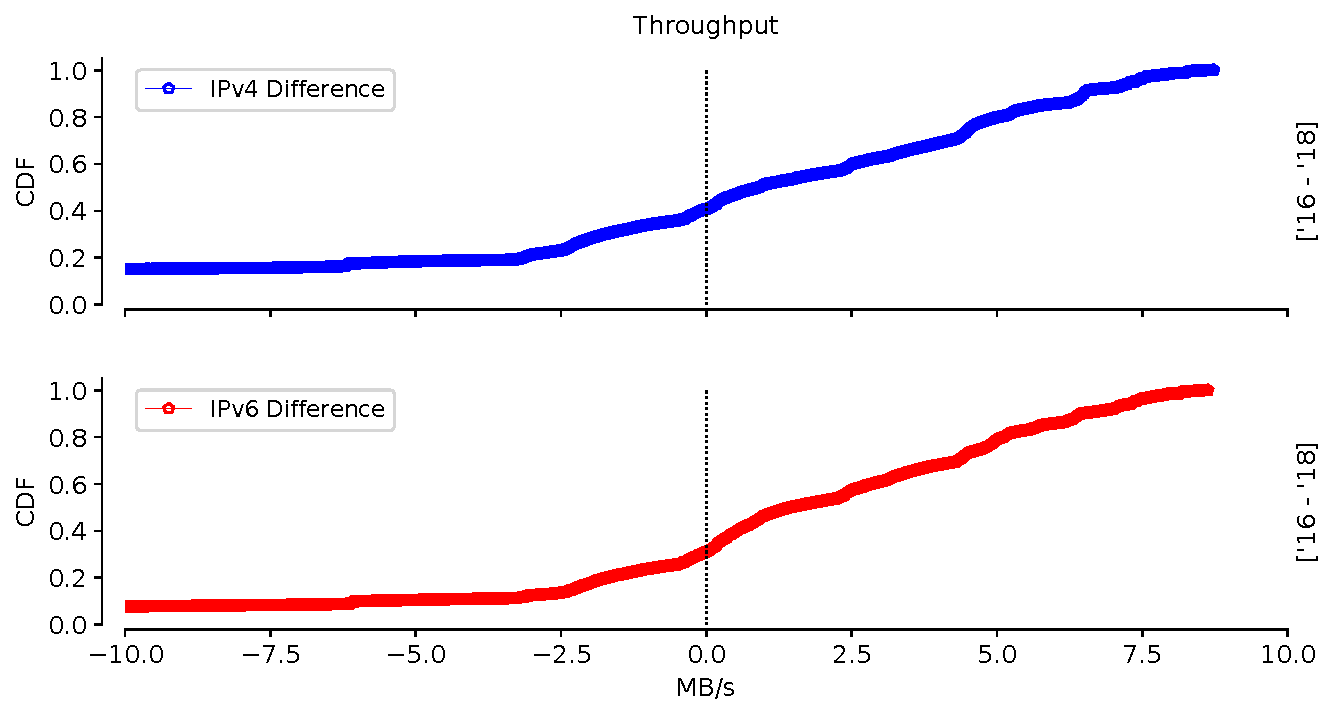
\includegraphics[keepaspectratio, height=5cm, width=15cm]{figures/cache/btuk/netflix-throughput-difference-2856.pdf}
	\caption[BT-UK Throughput CDF Deltas]{CDF of difference of throughput over IPv4 and IPv6 for BT and Netflix. 
Around 66\% of the times, BT caches achieved higher throughput than Netflix over IPv4 and IPv6.}
	\label{fig:BT-UK Throughput CDF Deltas}
\end{figure}

\FloatBarrier